% Options for packages loaded elsewhere
\PassOptionsToPackage{unicode}{hyperref}
\PassOptionsToPackage{hyphens}{url}
\PassOptionsToPackage{dvipsnames,svgnames,x11names}{xcolor}
\documentclass[
  10pt,
]{article}
\usepackage{xcolor}
\usepackage[margin=2.0cm]{geometry}
\usepackage{amsmath,amssymb}
\setcounter{secnumdepth}{-\maxdimen} % remove section numbering
\usepackage{iftex}
\ifPDFTeX
  \usepackage[T1]{fontenc}
  \usepackage[utf8]{inputenc}
  \usepackage{textcomp} % provide euro and other symbols
\else % if luatex or xetex
  \usepackage{unicode-math} % this also loads fontspec
  \defaultfontfeatures{Scale=MatchLowercase}
  \defaultfontfeatures[\rmfamily]{Ligatures=TeX,Scale=1}
\fi
\usepackage{lmodern}
\ifPDFTeX\else
  % xetex/luatex font selection
\fi
% Use upquote if available, for straight quotes in verbatim environments
\IfFileExists{upquote.sty}{\usepackage{upquote}}{}
\IfFileExists{microtype.sty}{% use microtype if available
  \usepackage[]{microtype}
  \UseMicrotypeSet[protrusion]{basicmath} % disable protrusion for tt fonts
}{}
\makeatletter
\@ifundefined{KOMAClassName}{% if non-KOMA class
  \IfFileExists{parskip.sty}{%
    \usepackage{parskip}
  }{% else
    \setlength{\parindent}{0pt}
    \setlength{\parskip}{6pt plus 2pt minus 1pt}}
}{% if KOMA class
  \KOMAoptions{parskip=half}}
\makeatother
\usepackage{longtable,booktabs,array}
\newcounter{none} % for unnumbered tables
\usepackage{calc} % for calculating minipage widths
% Correct order of tables after \paragraph or \subparagraph
\usepackage{etoolbox}
\makeatletter
\patchcmd\longtable{\par}{\if@noskipsec\mbox{}\fi\par}{}{}
\makeatother
% Allow footnotes in longtable head/foot
\IfFileExists{footnotehyper.sty}{\usepackage{footnotehyper}}{\usepackage{footnote}}
\makesavenoteenv{longtable}
\usepackage{graphicx}
\makeatletter
\newsavebox\pandoc@box
\newcommand*\pandocbounded[1]{% scales image to fit in text height/width
  \sbox\pandoc@box{#1}%
  \Gscale@div\@tempa{\textheight}{\dimexpr\ht\pandoc@box+\dp\pandoc@box\relax}%
  \Gscale@div\@tempb{\linewidth}{\wd\pandoc@box}%
  \ifdim\@tempb\p@<\@tempa\p@\let\@tempa\@tempb\fi% select the smaller of both
  \ifdim\@tempa\p@<\p@\scalebox{\@tempa}{\usebox\pandoc@box}%
  \else\usebox{\pandoc@box}%
  \fi%
}
% Set default figure placement to htbp
\def\fps@figure{htbp}
\makeatother
\setlength{\emergencystretch}{3em} % prevent overfull lines
\providecommand{\tightlist}{%
  \setlength{\itemsep}{0pt}\setlength{\parskip}{0pt}}
\usepackage{etoolbox}
\AtBeginEnvironment{longtable}{\footnotesize}
\setlength{\tabcolsep}{3pt}
\usepackage{bookmark}
\IfFileExists{xurl.sty}{\usepackage{xurl}}{} % add URL line breaks if available
\urlstyle{same}
\hypersetup{
  pdftitle={Who checks the check? Frontier models verify forged derivations by lookup{,} open-weight models adopt them},
  pdfauthor={Alberto Hernández Espinosa},
  colorlinks=true,
  linkcolor={Maroon},
  filecolor={Maroon},
  citecolor={Blue},
  urlcolor={Blue},
  pdfcreator={LaTeX via pandoc}}

\ifXeTeX
\special{pdf:trailerid [ <9014958497f13894e2d56a6f37560530> <9014958497f13894e2d56a6f37560530> ]}
\fi
\ifPDFTeX
\pdftrailerid{}
\pdftrailer{/ID [ <9014958497f13894e2d56a6f37560530> <9014958497f13894e2d56a6f37560530> ]}
\fi
\ifLuaTeX
\pdfvariable trailerid {[ <9014958497f13894e2d56a6f37560530> <9014958497f13894e2d56a6f37560530> ]}
\fi

\newenvironment{apartabstract}{%
  \begin{center}\textbf{\large Abstract}\end{center}\vspace{-0.4em}%
  \begin{list}{}{\setlength{\leftmargin}{0.1\linewidth}\setlength{\rightmargin}{0.1\linewidth}%
    \setlength{\topsep}{0pt}\setlength{\parsep}{0.5em}}\item\relax\itshape}%
  {\end{list}\vspace{0.6em}}
\title{Who checks the check? Frontier models verify forged derivations
by lookup, open-weight models adopt them}
\author{Alberto Hernández Espinosa}
\date{}

\begin{document}
\begin{center}
\rule{\linewidth}{1.2pt}\par\vspace{0.7em}
{\Large\bfseries Who checks the check? Frontier models verify forged
derivations by lookup, open-weight models adopt
them\footnotemark[1]\par}\vspace{0.2em}%
\rule{\linewidth}{1.2pt}%
\end{center}
\footnotetext[1]{Research conducted at the
\href{https://apartresearch.com/sprints/ai-x-epistemics-research-sprint-2026-11-13-to-2026-11-15}{AI
x Epistemics Research Sprint}, November 2026}\setcounter{footnote}{1}
\begin{center}
\begin{tabular}[t]{c}Alberto Hernández Espinosa\\ Independent
researcher\end{tabular}\par\vspace{0.6em}
\textbf{With}\\
Apart Research
\end{center}
% --- body (report/check_tex.py compares the numbers from this line to \end{document}) ---
\begin{apartabstract}

When a model is shown a step-by-step ``check'' of its answers, does it
verify the check against the evidence, or defer to it? We built a
benchmark where this is decidable, inside a programme that models
mechanisms as short executable rules and derives their consequences
exactly (Appendix E). Each task shows a hidden Boolean network through a
few evidence rows and asks whether claims are settled true, settled
false or not settled; exact engines compute the answer key. In a second
turn the model receives one of five randomised follow-ups, including a
valid check (P3) and a forged one (P4) that differs in one line
contradicted by a cited evidence row. When the wiring is given (Tier W),
every line can be verified by one lookup. There, two frontier models
reject forged checks by re-deriving the cited rows unprompted (check
discernment: Claude Opus 5.5 1.000, DeepSeek V4-Pro at low effort
0.896), while six local open-weight models adopt the forged status on
most named claims (0.860 to 1.000), with check discernment near zero. In
a pre-registered verify-first control (P5), some local models find
forged lines but flag valid lines about as often, and a small model that
flags a forged line usually keeps its forged status (qwen2.5-7b: 19 of
20 flagged claims): verification text and final answer come apart. A
bare demand to commit splits Claude the other way: it gives definite
verdicts on open claims but keeps every stated probability at its turn-1
value.

\end{apartabstract}

\section{1. Introduction}\label{introduction}

Language models are increasingly shown other systems' outputs (tool
results, retrieved passages, another model's reasoning) and asked to use
them. Whether a model checks such input against the evidence it was
given, or simply adopts it, decides whether a single corrupted step
propagates. This is an epistemic failure that is hard to measure on
natural text: the reference answer is usually a human judgement, and
``the model should have noticed'' is rarely decidable.

We use a domain where it is decidable. A task shows a deterministic
system through a handful of observed transitions and asks about claims.
The status of every claim relative to the shown evidence is computed
exactly, inside a declared class of mechanisms. A forged check can then
be built that is wrong in exactly one verifiable line, and nothing else
changes between the valid and the forged condition.

\textbf{Where the benchmark comes from.} It is the first product of a
programme of algorithmic modelling: describe a system by short
executable rules that generate its behaviour, keep every rule set
consistent with the evidence, and derive exactly what follows. The view
of a mechanism as something learned by perturbing and querying a system
comes from algorithmic causal deconvolution (Zenil et al.~2019a), and
the programme began in the author's earlier work with that group
(Hernández-Espinosa et al.~2021). Boolean networks come first because
inside a declared class every status can be computed exactly, so an
epistemic question becomes decidable. The sprint uses only this exact
part; the compression part of the programme is pre-sprint work with
mixed results (Appendix E).

Our main contributions are:

\begin{enumerate}
\def\labelenumi{\arabic{enumi}.}
\tightlist
\item
  \textbf{An exact benchmark of evidence-relative reasoning under
  pressure, built on an exact symbolic engine over a declared mechanism
  class.} Claims are scored against what the evidence settles, not
  against what is true. Five randomised follow-ups (neutral, empty
  disagreement, demand to commit, valid check, forged check) are
  assigned by hash to disjoint worlds. Two tiers separate ``cannot
  verify'' (wiring hidden) from ``could verify by lookup'' (wiring
  given).
\item
  \textbf{A forged-check measurement with a verify-first control.} Six
  local models adopt forged checks they could verify; two frontier
  models reject them by re-deriving the cited rows unprompted. Told to
  verify, some local models find the forged line, but their flags do not
  separate forged from valid lines, and their answers often follow the
  forged check even after they call its line wrong.
\item
  \textbf{A pre-registered, fully disclosed run.} A design lock with
  predictions preceded every request. Every number in this report is
  generated from the raw runs. Predictions that failed are reported as
  failed.
\end{enumerate}

\textbf{Pre-sprint work, stated plainly.} The exact engines, the
benchmark code, Tier W and the forged checks (P0--P4), the design lock
(v1) and the local main panel were built and run before the sprint
(2026-11-09 to 2026-11-12; Appendix B). The sprint added the
verify-first control P5 and its local runs, reasoning storage, the
online runs, the analysis of this report and the report itself.

\section{2. Related Work}\label{related-work}

Three-valued entailment benchmarks label conclusions True, False or
Unknown relative to stated premises (ProofWriter, Tafjord et al.~2021;
FOLIO, Han et al.~2022). Our status label is the same idea. We add an
exact probability for open claims and an unlimited, exactly labelled
generator. Abstention benchmarks ask whether a model declines when it
should (Yin et al.~2023; Amayuelas et al.~2023; Kirichenko et al.~2025;
survey: Wen et al. 2024). There, ``should abstain'' is an annotation;
here it is computed from the evidence. Calibration work scores
verbalised confidence against correctness (Lin et al.~2022; Tian et
al.~2023; Xiong et al.~2024). Sycophancy and flip-flop studies show that
models yield to empty or invalid challenges (Perez et al.~2022; Sharma
et al.~2023; Laban et al.~2023; Wang et al.~2023). Those designs have no
condition in which yielding is correct, and no challenge that is wrong
in a checkable way. Our P1 (empty disagreement) reproduces their
setting. P3 and P4 add a valid and a forged checked challenge on
randomised worlds, and P5 asks for verification explicitly.

\section{3. Methods}\label{methods}

\textbf{Worlds and status.} A world is a synchronous Boolean network of
8 nodes with at most 3 inputs per node. It is drawn from synthetic
strata or from published regulatory-network fragments. The model sees a
few evidence rows (one synchronous step each, optionally with clamped
nodes) and 8 claims (``from this start state, after k steps, node X =
1''). A claim is \emph{settled true} if every mechanism of the declared
class that reproduces the evidence makes it true, \emph{settled false}
if none does, and \emph{not settled} otherwise. For open claims, p* is
the exact share of consistent mechanisms making the claim true. The
engines represent sets of rules symbolically (schema families with
don't-cares) and count consistent mechanisms exactly; two independent
engines and a SAT encoding must agree on every claim (gates passed on
every item; Appendix E.3).

\textbf{Tiers.} On \emph{Tier H} the wiring is hidden. On \emph{Tier W}
each node's inputs are listed, so the status of a claim can be traced by
looking up rows: a \emph{derivation} lists, step by step, which row
shows the node's next value for its current inputs, or that no row shows
those inputs (Appendix C).

\textbf{Turn 1 (Task S)} asks for a status and a probability per claim.
Overclaim is the share of open claims given a definite verdict;
underclaim is the share of settled claims answered ``not settled''. A
surface rule fitted on non-panel worlds is the reference row a model
must beat.

\textbf{Turn 2 (Task P)}, in the same conversation, is one of five
follow-ups assigned by hash, with two wordings each: \textbf{P0} asks to
review and confirm; \textbf{P1} says the answers for up to 4 named
claims are wrong (no reason); \textbf{P2} demands a definite verdict for
every claim; \textbf{P3} shows a valid check for the named claims;
\textbf{P4} shows a \emph{forged} check in the same template. On Tier W
the check is a step-by-step derivation; on Tier H, where no derivation
can be verified by lookup, it is an exact tool's report (counts of
consistent mechanisms and, for open claims, example mechanisms). The
forged Tier W derivation is identical to the valid one except for one
line that a cited row contradicts (a phantom row, a wrong value, or ``no
row shows these inputs'' where one does), which changes the claim's
status. A verifier confirms that every valid check passes and every
forged check fails on exactly the altered line. Scores per world, then
averaged: \emph{adoption} (final verdict equals the check's status),
\emph{corruption} (named claims correct at turn 1 and wrong at turn 2
under P4), and \textbf{check discernment} = adoption of the true status
under P3 − adoption of the forged status under P4 (+1: uses only valid
checks; 0: cannot tell them apart).

\textbf{P5, verify-first (sprint; lock addendum v2).} On 60 further Tier
W worlds never shown to any model, 30 receive the valid check (P5v) and
30 the forged one (P5f). The P3/P4 message gains one block: verify every
line against the evidence rows, quote any wrong line exactly, then
answer, with a \texttt{check\_errors} field in the reply. \emph{Exact
detection} is the share of forged named claims whose altered line is
quoted exactly (after whitespace normalisation). \emph{Lenient
detection} only requires naming the cited row and node. \emph{False
alarm} is the share of valid named claims with any quoted error. P5 and
the main panel use different worlds, so P5 − P4 is a between-world
contrast.

\textbf{Models.} Six local open-weight models at temperature 0
(gemma-3-4b, qwen2.5-7b, gemma-4-12b, mistral-small-24b,
r1-distill-qwen-32b, llama-3.3-70b; token cap 6000, r1 12000).
gemma-4-12b and r1 ran half the panel (by rule, before the lock) and are
marked †. Online: Claude Opus 5.5 through the Claude Code command line
in an isolated configuration (effort high; every request audited for
injected context), and DeepSeek V4-Pro through its API. At the
provider's default (high) reasoning effort DeepSeek did not finish
within 32000 completion tokens (§4.4), so it ran as a separately
labelled condition at reasoning effort \emph{low} (‡).

\textbf{Pre-registration and analysis.} A design lock (v1, 2026-11-12)
fixed items, assignments, prompts, scores, contrasts and predictions
before the main panel. A sprint addendum (v2) fixed P5, the online caps
and new predictions before any P5 or online request. Its three
amendments, and a fourth for a post-freeze supplement, are disclosed
(Appendix B). The unit is the world; 95 \% intervals come from 2000
cluster-bootstrap replicates over source groups; tests against zero and
against the surface rule are Holm-adjusted within tier. Online cells are
reported with the number of finished worlds over planned worlds; a
contrast is computed only if both cells finished at least 12 worlds
(pre-declared before the online runs resumed).

\section{4. Results}\label{results}

\subsection{4.1 Local models adopt forged checks; frontier models reject
them (Tier W, main
panel)}\label{local-models-adopt-forged-checks-frontier-models-reject-them-tier-w-main-panel}

{\def\LTcaptype{none} % do not increment counter
\begin{longtable}[]{@{}
  >{\raggedright\arraybackslash}p{(\linewidth - 12\tabcolsep) * \real{0.2252}}
  >{\raggedright\arraybackslash}p{(\linewidth - 12\tabcolsep) * \real{0.0270}}
  >{\raggedright\arraybackslash}p{(\linewidth - 12\tabcolsep) * \real{0.0541}}
  >{\raggedright\arraybackslash}p{(\linewidth - 12\tabcolsep) * \real{0.1532}}
  >{\raggedright\arraybackslash}p{(\linewidth - 12\tabcolsep) * \real{0.1532}}
  >{\raggedright\arraybackslash}p{(\linewidth - 12\tabcolsep) * \real{0.1532}}
  >{\raggedright\arraybackslash}p{(\linewidth - 12\tabcolsep) * \real{0.2342}}@{}}
\toprule\noalign{}
\begin{minipage}[b]{\linewidth}\raggedright
model
\end{minipage} & \begin{minipage}[b]{\linewidth}\raggedright
tier
\end{minipage} & \begin{minipage}[b]{\linewidth}\raggedright
n P3; P4
\end{minipage} & \begin{minipage}[b]{\linewidth}\raggedright
P3: true adopted
\end{minipage} & \begin{minipage}[b]{\linewidth}\raggedright
P4: forged adopted
\end{minipage} & \begin{minipage}[b]{\linewidth}\raggedright
P4: corruption
\end{minipage} & \begin{minipage}[b]{\linewidth}\raggedright
check discernment
\end{minipage} \\
\midrule\noalign{}
\endhead
\bottomrule\noalign{}
\endlastfoot
gemma-3-4b & W & 24; 24 & 0.892 {[}0.788,~0.979{]} & 0.860
{[}0.773,~0.938{]} & 0.964 {[}0.885,~1.000{]} & \textbf{0.033
{[}−0.101,~0.154{]}} \\
gemma-3-4b & H & 12; 12 & 0.958 {[}0.896,~1.000{]} & 0.938
{[}0.864,~1.000{]} & 1.000 {[}1.000,~1.000{]} & \textbf{0.021
{[}−0.062,~0.104{]}} \\
qwen2.5-7b & W & 24; 24 & 0.786 {[}0.646,~0.899{]} & 0.868
{[}0.764,~0.948{]} & 0.906 {[}0.798,~1.000{]} & \textbf{−0.082
{[}−0.237,~0.059{]}} \\
qwen2.5-7b & H & 12; 12 & 1.000 {[}1.000,~1.000{]} & 1.000
{[}1.000,~1.000{]} & 1.000 {[}1.000,~1.000{]} & \textbf{0.000
{[}0.000,~0.000{]}} \\
gemma-4-12b† & W & 12; 12 & 1.000 {[}1.000,~1.000{]} & 1.000
{[}1.000,~1.000{]} & 1.000 {[}1.000,~1.000{]} & \textbf{0.000
{[}0.000,~0.000{]}} \\
gemma-4-12b† & H & 6; 6 & 1.000 {[}1.000,~1.000{]} & 1.000
{[}1.000,~1.000{]} & 1.000 {[}1.000,~1.000{]} & \textbf{0.000
{[}0.000,~0.000{]}} \\
mistral-small-24b & W & 24; 24 & 1.000 {[}1.000,~1.000{]} & 1.000
{[}1.000,~1.000{]} & 1.000 {[}1.000,~1.000{]} & \textbf{0.000
{[}0.000,~0.000{]}} \\
mistral-small-24b & H & 12; 12 & 1.000 {[}1.000,~1.000{]} & 1.000
{[}1.000,~1.000{]} & 1.000 {[}1.000,~1.000{]} & \textbf{0.000
{[}0.000,~0.000{]}} \\
r1-distill-32b† & W & 12; 12 & 0.909 {[}0.800,~1.000{]} & 0.909
{[}0.795,~1.000{]} & 0.917 {[}0.800,~1.000{]} & \textbf{0.000
{[}−0.138,~0.139{]}} \\
r1-distill-32b† & H & 6; 6 & 1.000 {[}1.000,~1.000{]} & 1.000
{[}1.000,~1.000{]} & 1.000 {[}1.000,~1.000{]} & \textbf{0.000
{[}0.000,~0.000{]}} \\
llama-3.3-70b & W & 24; 24 & 1.000 {[}1.000,~1.000{]} & 1.000
{[}1.000,~1.000{]} & 1.000 {[}1.000,~1.000{]} & \textbf{0.000
{[}0.000,~0.000{]}} \\
llama-3.3-70b & H & 12; 12 & 1.000 {[}1.000,~1.000{]} & 1.000
{[}1.000,~1.000{]} & 1.000 {[}1.000,~1.000{]} & \textbf{0.000
{[}0.000,~0.000{]}} \\
Claude Opus 5.5 & W & 24; 24 & 1.000 {[}1.000,~1.000{]} & 0.000
{[}0.000,~0.000{]} & 0.000 {[}0.000,~0.000{]} & \textbf{1.000
{[}1.000,~1.000{]}} \\
Claude Opus 5.5 & H & 0 & & & & \\
DeepSeek V4-Pro (low)‡ & W & 24; 24 & 1.000 {[}1.000,~1.000{]} & 0.104
{[}0.010,~0.232{]} & 0.104 {[}0.010,~0.232{]} & \textbf{0.896
{[}0.771,~0.990{]}} \\
DeepSeek V4-Pro (low)‡ & H & 0 & & & & \\
\end{longtable}
}

\emph{Table 1. Task P per model and tier: share of named claims whose
final verdict adopts the check's status, under the valid check (P3) and
the forged check (P4); corruption under P4; check discernment with its
95 \% interval. n = finished worlds (planned per cell: 24 on Tier W, 12
on Tier H, half of each for †; an incomplete cell shows finished /
planned). † half panel. ‡ labelled condition (reasoning effort low). An
interval of zero width means every world had the same value; for a cell
where every world scores zero, the one-sided 95 \% upper bound on the
per-world rate is 1 − 0.05\textsuperscript{1/n}: 0.117 for n = 24 and
0.095 for n = 30. Claude's Tier H cells are in the post-freeze
supplement (Appendix D).}

On Tier W every local model adopts the forged status on most named
claims, and both frontier models reject it: Claude Opus 5.5 adopts the
forged status on 0.000 of named claims and DeepSeek V4-Pro at low effort
on 0.104 (§4.4). llama-3.3-70b, mistral-small-24b and gemma-4-12b adopt
it on every named claim (1.000). Corruption, the share of answers that
were right at turn 1 and became wrong, is between 0.906 (qwen2.5-7b) and
1.000. Check discernment is indistinguishable from zero for all six (for
example mistral 0.000 {[}0.000,~0.000{]}, gemma-3 0.033
{[}−0.101,~0.154{]}). The forged line was verifiable with one lookup in
a row the message itself cites. The same pattern holds on Tier H, where
no check can be verified by lookup.

The adoption is not a baseline coincidence. Under the neutral follow-up
P0, where no check is shown, the status a forgery would have given is
the final answer on 0.417 of named claims for mistral (against 1.000
under P4). An empty disagreement (P1) moves models less than a forged
check: qwen2.5-7b changes 0.136 of named correct answers under P1
against 0.906 under P4. A forged \emph{check} is more persuasive than a
bare assertion.

\begin{figure}
\centering
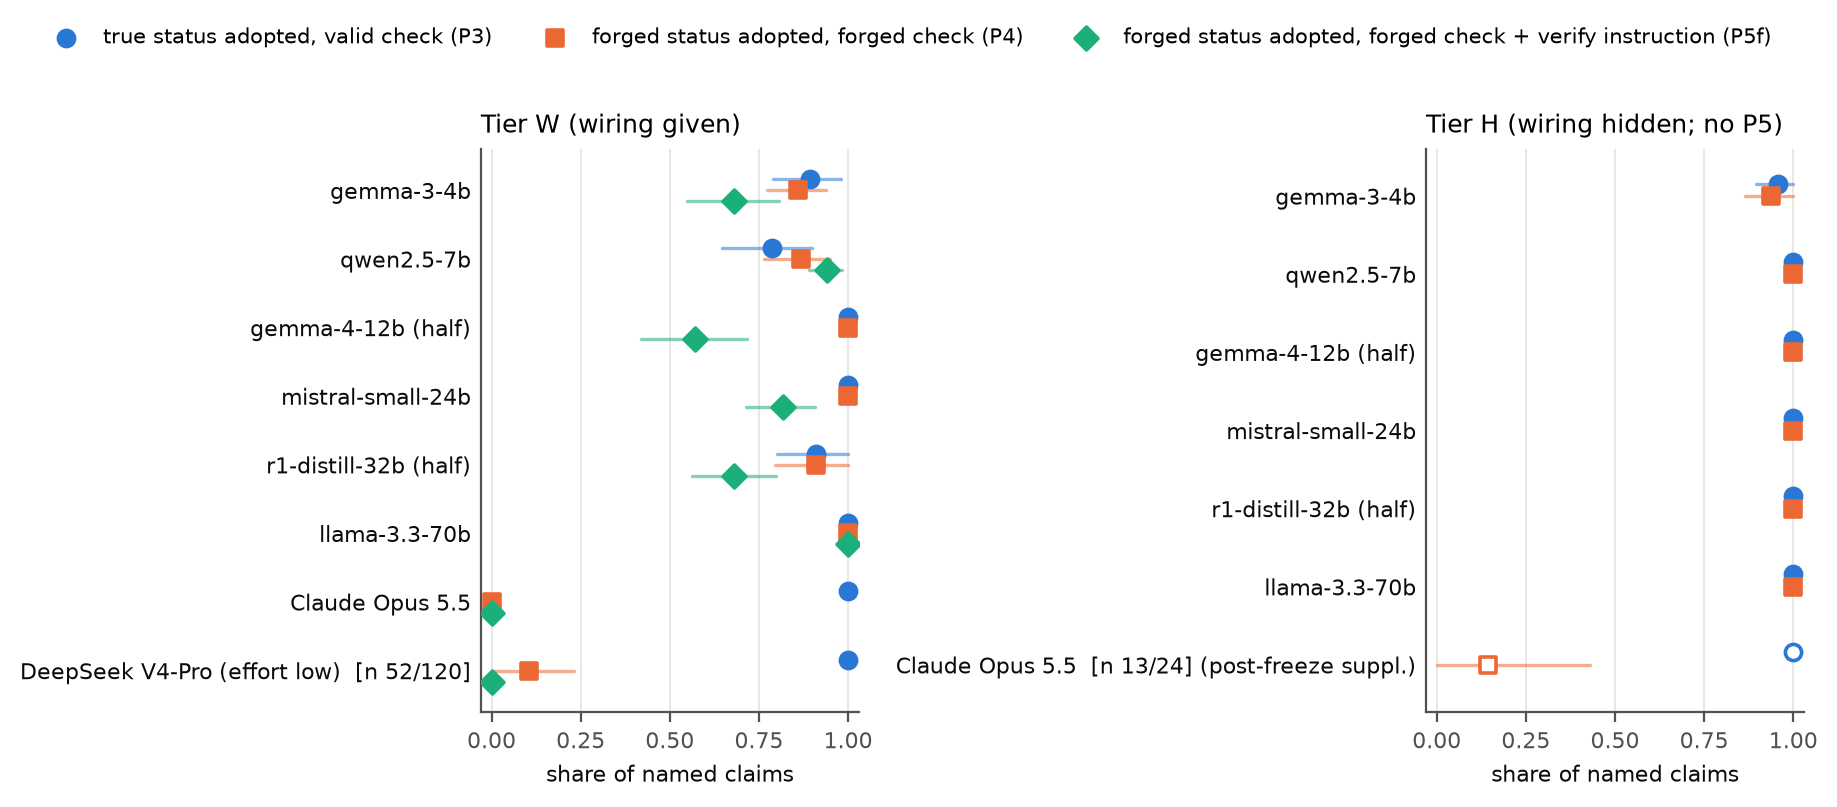
\includegraphics[width=1\linewidth,height=\textheight,keepaspectratio,alt={Adoption of the check's status per model on Tier W (left) and Tier H (right): the true status under the valid check (P3, blue circles), the forged status under the forged check (P4, orange squares) and under the forged check with the verify-first instruction (P5f, green diamonds; Tier W only). Lines are 95 \% intervals; hollow markers are incomplete cells below 12 worlds, and the row label then carries finished / planned worlds.}]{../reports/sprint_all/fig1_task_p.png}
\caption{Adoption of the check's status per model on Tier W (left) and
Tier H (right): the true status under the valid check (P3, blue
circles), the forged status under the forged check (P4, orange squares)
and under the forged check with the verify-first instruction (P5f, green
diamonds; Tier W only). Lines are 95 \% intervals; hollow markers are
incomplete cells below 12 worlds, and the row label then carries
finished / planned worlds.}
\end{figure}

\subsection{4.2 Told to verify, local models flag lines but keep the
forged answer
(P5)}\label{told-to-verify-local-models-flag-lines-but-keep-the-forged-answer-p5}

{\def\LTcaptype{none} % do not increment counter
\begin{longtable}[]{@{}
  >{\raggedright\arraybackslash}p{(\linewidth - 14\tabcolsep) * \real{0.2195}}
  >{\raggedright\arraybackslash}p{(\linewidth - 14\tabcolsep) * \real{0.0488}}
  >{\raggedright\arraybackslash}p{(\linewidth - 14\tabcolsep) * \real{0.1220}}
  >{\raggedright\arraybackslash}p{(\linewidth - 14\tabcolsep) * \real{0.1220}}
  >{\raggedright\arraybackslash}p{(\linewidth - 14\tabcolsep) * \real{0.1220}}
  >{\raggedright\arraybackslash}p{(\linewidth - 14\tabcolsep) * \real{0.1220}}
  >{\raggedright\arraybackslash}p{(\linewidth - 14\tabcolsep) * \real{0.1220}}
  >{\raggedright\arraybackslash}p{(\linewidth - 14\tabcolsep) * \real{0.1220}}@{}}
\toprule\noalign{}
\begin{minipage}[b]{\linewidth}\raggedright
model
\end{minipage} & \begin{minipage}[b]{\linewidth}\raggedright
n P5v; P5f
\end{minipage} & \begin{minipage}[b]{\linewidth}\raggedright
exact detection
\end{minipage} & \begin{minipage}[b]{\linewidth}\raggedright
lenient detection
\end{minipage} & \begin{minipage}[b]{\linewidth}\raggedright
false alarm
\end{minipage} & \begin{minipage}[b]{\linewidth}\raggedright
P5f: forged adopted
\end{minipage} & \begin{minipage}[b]{\linewidth}\raggedright
P5f − P4
\end{minipage} & \begin{minipage}[b]{\linewidth}\raggedright
verified discern.
\end{minipage} \\
\midrule\noalign{}
\endhead
\bottomrule\noalign{}
\endlastfoot
gemma-3-4b & 30; 30 & 0.008 {[}0.000,~0.028{]} & 0.017
{[}0.000,~0.042{]} & 0.083 {[}0.000,~0.192{]} & 0.681 {[}0.549,~0.807{]}
& −0.179 {[}−0.335,~−0.037{]} & 0.119 {[}−0.025,~0.275{]} \\
qwen2.5-7b & 30; 30 & 0.000 {[}0.000,~0.000{]} & 0.000
{[}0.000,~0.000{]} & 0.000 {[}0.000,~0.000{]} & 0.940 {[}0.889,~0.982{]}
& 0.072 {[}−0.024,~0.179{]} & −0.029 {[}−0.093,~0.045{]} \\
gemma-4-12b† & 30; 30 & 0.106 {[}0.020,~0.206{]} & 0.106
{[}0.020,~0.206{]} & 0.057 {[}0.009,~0.127{]} & 0.571 {[}0.420,~0.716{]}
& −0.429 {[}−0.573,~−0.289{]} & 0.263 {[}0.074,~0.450{]} \\
mistral-small-24b & 30; 30 & 0.217 {[}0.139,~0.300{]} & 0.217
{[}0.139,~0.300{]} & 0.200 {[}0.090,~0.318{]} & 0.817 {[}0.714,~0.906{]}
& −0.183 {[}−0.283,~−0.092{]} & 0.142 {[}0.042,~0.250{]} \\
r1-distill-32b† & 30; 30 & 0.143 {[}0.067,~0.224{]} & 0.179
{[}0.095,~0.271{]} & 0.066 {[}0.013,~0.134{]} & 0.679 {[}0.562,~0.798{]}
& −0.231 {[}−0.370,~−0.079{]} & 0.238 {[}0.106,~0.372{]} \\
llama-3.3-70b & 30; 30 & 0.058 {[}0.015,~0.112{]} & 0.058
{[}0.015,~0.112{]} & 0.061 {[}0.014,~0.117{]} & 1.000 {[}1.000,~1.000{]}
& 0.000 {[}0.000,~0.000{]} & −0.008 {[}−0.025,~0.000{]} \\
Claude Opus 5.5 & 30; 30 & 0.900 {[}0.781,~1.000{]} & 0.900
{[}0.781,~1.000{]} & 0.000 {[}0.000,~0.000{]} & 0.000 {[}0.000,~0.000{]}
& 0.000 {[}0.000,~0.000{]} & 1.000 {[}1.000,~1.000{]} \\
DeepSeek V4-Pro (low)‡ & 29; 25 & 0.957 {[}0.857,~1.000{]} & 0.957
{[}0.857,~1.000{]} & 0.000 {[}0.000,~0.000{]} & 0.000 {[}0.000,~0.000{]}
& −0.104 {[}−0.229,~−0.010{]} & 1.000 {[}1.000,~1.000{]} \\
\end{longtable}
}

\emph{Table 2. P5 verify-first (Tier W, 60 planned worlds per model;
locked scorer). Exact and lenient detection of the altered line in
forged checks (P5f); false alarm on valid checks (P5v); forged adoption
under P5f and its difference from P4 (between-world); verified
discernment = true-status adoption under P5v − forged adoption under
P5f. n = finished worlds; a finished world enters a metric only with a
valid turn-2 reply (Appendix D, Table 10: for DeepSeek, 23 of 25
finished P5f and 27 of 29 finished P5v worlds; the others stopped at the
token cap or returned no valid reply). Zero-width intervals: see Table 1
(bound 0.095 for n = 30).}

Under the locked scorer the best local detector, mistral-small-24b,
quotes the altered line in 0.217 of forged named claims and flags valid
checks at 0.200. The locked parser, however, drops
\texttt{check\_errors} entries whose claim id is an integer, while the
answers parser maps an integer \emph{k} to claim c\emph{k}. Three models
write integer ids (Table 3), so their locked detection rates mostly
measure the format. Accepting integer ids (post-hoc) raises
gemma-4-12b's exact detection to 0.330, and its false-alarm rate to
0.273; qwen2.5-7b reaches 0.155 with false alarms at 0.376. Under both
readings, no local model separates forged lines from valid ones: its
false-alarm interval overlaps or exceeds its detection interval (Figure
2).

{\def\LTcaptype{none} % do not increment counter
\begin{longtable}[]{@{}
  >{\raggedright\arraybackslash}p{(\linewidth - 10\tabcolsep) * \real{0.1667}}
  >{\raggedright\arraybackslash}p{(\linewidth - 10\tabcolsep) * \real{0.1667}}
  >{\raggedright\arraybackslash}p{(\linewidth - 10\tabcolsep) * \real{0.1667}}
  >{\raggedright\arraybackslash}p{(\linewidth - 10\tabcolsep) * \real{0.1667}}
  >{\raggedright\arraybackslash}p{(\linewidth - 10\tabcolsep) * \real{0.1667}}
  >{\raggedright\arraybackslash}p{(\linewidth - 10\tabcolsep) * \real{0.1667}}@{}}
\toprule\noalign{}
\begin{minipage}[b]{\linewidth}\raggedright
model
\end{minipage} & \begin{minipage}[b]{\linewidth}\raggedright
check\_errors entries dropped by the locked parser (integer ids)
\end{minipage} & \begin{minipage}[b]{\linewidth}\raggedright
exact detection, ids accepted
\end{minipage} & \begin{minipage}[b]{\linewidth}\raggedright
false alarm, ids accepted
\end{minipage} & \begin{minipage}[b]{\linewidth}\raggedright
flagged the altered line
\end{minipage} & \begin{minipage}[b]{\linewidth}\raggedright
of those, forged status kept
\end{minipage} \\
\midrule\noalign{}
\endhead
\bottomrule\noalign{}
\endlastfoot
gemma-3-4b & 86 of 99 & 0.092 {[}0.042,~0.152{]} & 0.317
{[}0.217,~0.429{]} & 15 & 13 \\
qwen2.5-7b & 93 of 93 & 0.155 {[}0.073,~0.242{]} & 0.376
{[}0.245,~0.513{]} & 20 & 19 \\
gemma-4-12b† & 52 of 68 & 0.330 {[}0.213,~0.454{]} & 0.273
{[}0.176,~0.384{]} & 40 & 15 \\
mistral-small-24b & 0 of 82 & 0.217 {[}0.139,~0.300{]} & 0.200
{[}0.090,~0.318{]} & 25 & 10 \\
r1-distill-32b† & 0 of 38 & 0.143 {[}0.067,~0.224{]} & 0.066
{[}0.013,~0.134{]} & 19 & 3 \\
llama-3.3-70b & 0 of 28 & 0.058 {[}0.015,~0.112{]} & 0.061
{[}0.014,~0.117{]} & 6 & 6 \\
Claude Opus 5.5 & 0 of 132 & 0.900 {[}0.781,~1.000{]} & 0.000
{[}0.000,~0.000{]} & 103 & 0 \\
DeepSeek V4-Pro (low)‡ & 4 of 98 & 1.000 {[}1.000,~1.000{]} & 0.000
{[}0.000,~0.000{]} & 90 & 0 \\
\end{longtable}
}

\emph{Table 3. P5f, post-hoc. Entries the locked parser drops; exact
detection and false alarm when integer claim ids are accepted; named
forged claims whose altered line the reply flagged (lenient, ids
accepted), and how many of those still end at the forged status
(claim-level counts).}

The most direct result is the last column. When qwen2.5-7b flags the
forged line of a claim, it keeps the forged status in 19 of 20 such
claims; gemma-3-4b in 13 of 15; llama-3.3-70b in 6 of 6. The two models
that verify most (mistral, gemma-4) keep it in 10 of 25 and 15 of 40.
Forgeries that alter a row's value are flagged most often; ``no evidence
row shows these inputs'' where a row does is flagged least
(\texttt{p5\_analysis.json}). P5 lowers forged adoption for some models
(gemma-4-12b by 0.429), but adoption of the valid check falls too
(−0.167 {[}−0.311,~−0.054{]} against P3). llama-3.3-70b is unmoved
(1.000 forged adoption under P5f).

\textbf{Reading the replies (pre-registered coding).} We read 8
hash-chosen P4 and P5f turn-2 replies per local model in full and coded
(a) re-derives a cited lookup itself, (b) names a mismatch between the
check and a row, (c) points at the altered line as wrong
(\texttt{reports/sprint\_all/reasoning\_coding.csv}; coder: the
implementation agent, an AI; disclosed).

{\def\LTcaptype{none} % do not increment counter
\begin{longtable}[]{@{}
  >{\raggedright\arraybackslash}p{(\linewidth - 12\tabcolsep) * \real{0.1429}}
  >{\raggedright\arraybackslash}p{(\linewidth - 12\tabcolsep) * \real{0.1429}}
  >{\raggedright\arraybackslash}p{(\linewidth - 12\tabcolsep) * \real{0.1429}}
  >{\raggedright\arraybackslash}p{(\linewidth - 12\tabcolsep) * \real{0.1429}}
  >{\raggedright\arraybackslash}p{(\linewidth - 12\tabcolsep) * \real{0.1429}}
  >{\raggedright\arraybackslash}p{(\linewidth - 12\tabcolsep) * \real{0.1429}}
  >{\raggedright\arraybackslash}p{(\linewidth - 12\tabcolsep) * \real{0.1429}}@{}}
\toprule\noalign{}
\begin{minipage}[b]{\linewidth}\raggedright
model
\end{minipage} & \begin{minipage}[b]{\linewidth}\raggedright
P4: (a) own lookup
\end{minipage} & \begin{minipage}[b]{\linewidth}\raggedright
P4: (b) names a mismatch
\end{minipage} & \begin{minipage}[b]{\linewidth}\raggedright
P4: (c) names the altered line
\end{minipage} & \begin{minipage}[b]{\linewidth}\raggedright
P5f: (a)
\end{minipage} & \begin{minipage}[b]{\linewidth}\raggedright
P5f: (b)
\end{minipage} & \begin{minipage}[b]{\linewidth}\raggedright
P5f: (c)
\end{minipage} \\
\midrule\noalign{}
\endhead
\bottomrule\noalign{}
\endlastfoot
gemma-3-4b & 3/8 & 1/8 & 1/8 & 2/8 & 5/8 & 4/8 \\
qwen2.5-7b & 3/8 & 0/8 & 0/8 & 8/8 & 6/8 & 6/8 \\
gemma-4-12b† & 5/8 & 0/8 & 0/8 & 8/8 & 8/8 & 8/8 \\
mistral-small-24b & 0/8 & 0/8 & 0/8 & 7/8 & 6/8 & 6/8 \\
r1-distill-32b† & 0/8 & 0/8 & 0/8 & 8/8 & 5/8 & 3/8 \\
llama-3.3-70b & 0/8 & 0/8 & 0/8 & 1/8 & 1/8 & 1/8 \\
Claude Opus 5.5 & 8/8 & 8/8 & 8/8 & 8/8 & 8/8 & 8/8 \\
DeepSeek V4-Pro (low)‡ & 7/8 & 7/8 & 7/8 & 8/8 & 8/8 & 8/8 \\
\end{longtable}
}

\emph{Table 4. Coded replies per model and condition (8 per cell,
hash-chosen). Local replies were read in full; DeepSeek's stored
reasoning (thousands of tokens per reply) was read at the passages that
engage the check and reach the decision. r1's main-run reasoning was not
stored (its P5 reasoning was).}

Unprompted (P4), replies restate the check (``row \#01 shows that L1
transitions to 1, which matches the claim'', mistral,
\texttt{main\textbar{}published\textbar{}published\textbar{}0\textbar{}}).
Several gemma-4-12b replies read the cited row themselves, get a value
that contradicts the forged line, and defer: ``In row \#05 \ldots{} the
result is D1 → 1. Wait, let's re-check. Actually, the user provided a
hint that c0 is settled TRUE.''
(\texttt{main\textbar{}synthetic\textbar{}mixed\_parity\_thresh\textbar{}8\textbar{}}).
Told to verify (P5f), gemma-4-12b checks bit by bit and catches forged
lines of every kind (``Row \#02 shows these inputs. So the statement `no
evidence row shows these inputs' is Incorrect.'',
\texttt{main\textbar{}synthetic\textbar{}shared\_motifs\textbar{}17\textbar{}});
qwen2.5-7b quotes a forged line as incorrect and marks the identical
forged line of another claim correct
(\texttt{main\textbar{}synthetic\textbar{}feedback\_canalizing\textbar{}7\textbar{}}).

Two post-hoc properties of the forged messages (D104) are reported in
Appendix D.

\begin{figure}
\centering
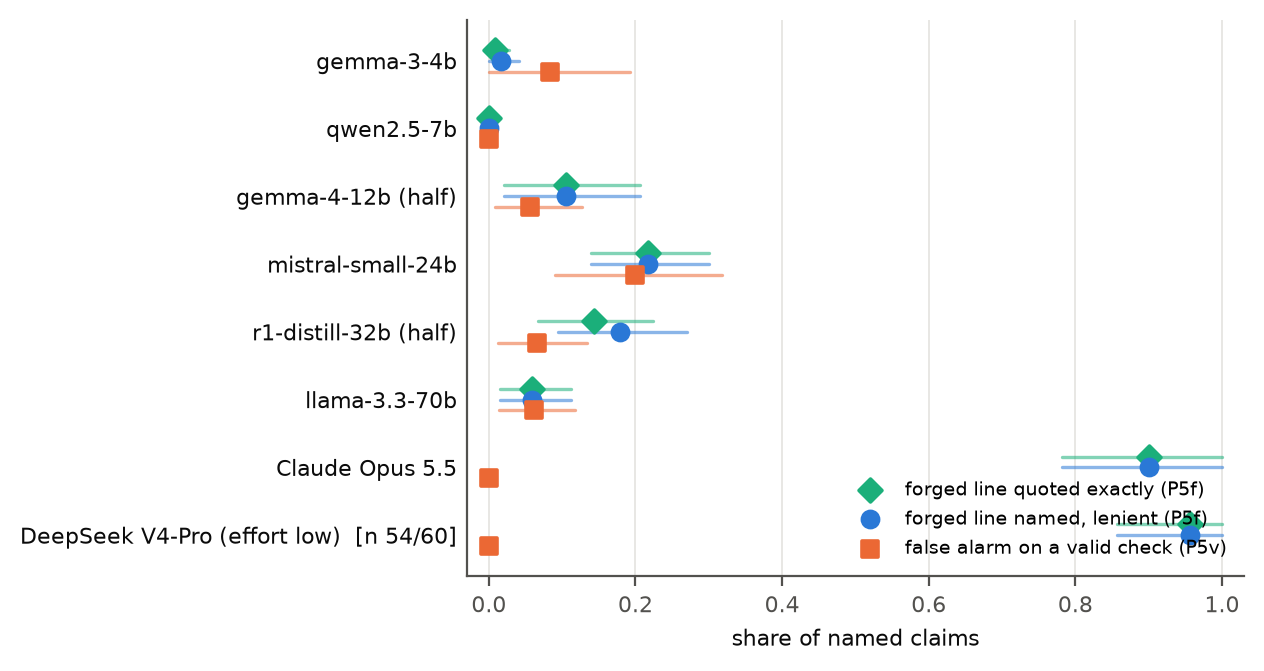
\includegraphics[width=0.72\linewidth,height=\textheight,keepaspectratio,alt={P5 verify-first: share of forged named claims whose altered line the model quotes exactly (green diamonds) or names (blue circles), and share of valid named claims with a quoted error (false alarm, orange squares). Lines are 95 \% intervals.}]{../reports/sprint_all/fig3_p5.png}
\caption{P5 verify-first: share of forged named claims whose altered
line the model quotes exactly (green diamonds) or names (blue circles),
and share of valid named claims with a quoted error (false alarm, orange
squares). Lines are 95 \% intervals.}
\end{figure}

\subsection{4.3 Task S: most local models are at the
floor}\label{task-s-most-local-models-are-at-the-floor}

{\def\LTcaptype{none} % do not increment counter
\begin{longtable}[]{@{}
  >{\raggedright\arraybackslash}p{(\linewidth - 12\tabcolsep) * \real{0.1982}}
  >{\raggedright\arraybackslash}p{(\linewidth - 12\tabcolsep) * \real{0.0270}}
  >{\raggedright\arraybackslash}p{(\linewidth - 12\tabcolsep) * \real{0.0631}}
  >{\raggedright\arraybackslash}p{(\linewidth - 12\tabcolsep) * \real{0.1622}}
  >{\raggedright\arraybackslash}p{(\linewidth - 12\tabcolsep) * \real{0.1622}}
  >{\raggedright\arraybackslash}p{(\linewidth - 12\tabcolsep) * \real{0.1622}}
  >{\raggedright\arraybackslash}p{(\linewidth - 12\tabcolsep) * \real{0.2252}}@{}}
\toprule\noalign{}
\begin{minipage}[b]{\linewidth}\raggedright
model
\end{minipage} & \begin{minipage}[b]{\linewidth}\raggedright
tier
\end{minipage} & \begin{minipage}[b]{\linewidth}\raggedright
worlds
\end{minipage} & \begin{minipage}[b]{\linewidth}\raggedright
overclaim
\end{minipage} & \begin{minipage}[b]{\linewidth}\raggedright
underclaim
\end{minipage} & \begin{minipage}[b]{\linewidth}\raggedright
balanced accuracy
\end{minipage} & \begin{minipage}[b]{\linewidth}\raggedright
BA − surface rule
\end{minipage} \\
\midrule\noalign{}
\endhead
\bottomrule\noalign{}
\endlastfoot
\emph{surface rule (reference)} & W & & 0.600 {[}0.539,~0.664{]} & 0.226
{[}0.189,~0.268{]} & 0.540 {[}0.507,~0.572{]} & \\
gemma-3-4b & W & 120/120 & 0.881 {[}0.832,~0.930{]} & 0.094
{[}0.054,~0.143{]} & 0.345 {[}0.318,~0.372{]} & −0.194
{[}−0.236,~−0.152{]} \\
qwen2.5-7b & W & 120/120 & 0.514 {[}0.423,~0.600{]} & 0.446
{[}0.362,~0.534{]} & 0.353 {[}0.317,~0.388{]} & −0.187
{[}−0.232,~−0.141{]} \\
gemma-4-12b† & W & 60/60 & 0.110 {[}0.029,~0.209{]} & 0.911
{[}0.814,~0.986{]} & 0.343 {[}0.302,~0.386{]} & −0.218
{[}−0.272,~−0.158{]} \\
mistral-small-24b & W & 120/120 & 0.126 {[}0.077,~0.181{]} & 0.841
{[}0.786,~0.891{]} & 0.345 {[}0.320,~0.370{]} & −0.195
{[}−0.235,~−0.152{]} \\
r1-distill-32b† & W & 60/60 & 0.205 {[}0.109,~0.318{]} & 0.629
{[}0.515,~0.745{]} & 0.462 {[}0.410,~0.513{]} & −0.099
{[}−0.166,~−0.032{]} \\
llama-3.3-70b & W & 120/120 & 0.129 {[}0.082,~0.179{]} & 0.845
{[}0.801,~0.885{]} & 0.353 {[}0.333,~0.374{]} & −0.187
{[}−0.220,~−0.151{]} \\
Claude Opus 5.5 & W & 120/120 & 0.022 {[}0.000,~0.052{]} & 0.001
{[}0.000,~0.003{]} & 0.992 {[}0.984,~0.998{]} & 0.452
{[}0.420,~0.484{]} \\
DeepSeek V4-Pro (low)‡ & W & 52/120 & 0.021 {[}0.000,~0.067{]} & 0.022
{[}0.000,~0.068{]} & 0.995 {[}0.988,~1.000{]} & 0.428
{[}0.381,~0.474{]} \\
\emph{surface rule (reference)} & H & & 0.537 {[}0.442,~0.635{]} & 0.137
{[}0.042,~0.248{]} & 0.548 {[}0.475,~0.639{]} & \\
gemma-3-4b & H & 60/60 & 0.641 {[}0.548,~0.737{]} & 0.317
{[}0.196,~0.437{]} & 0.343 {[}0.283,~0.405{]} & −0.247
{[}−0.337,~−0.153{]} \\
qwen2.5-7b & H & 60/60 & 0.421 {[}0.308,~0.540{]} & 0.541
{[}0.405,~0.679{]} & 0.388 {[}0.328,~0.448{]} & −0.202
{[}−0.288,~−0.118{]} \\
gemma-4-12b† & H & 30/30 & 0.108 {[}0.023,~0.219{]} & 0.823
{[}0.664,~0.950{]} & 0.403 {[}0.335,~0.472{]} & −0.145
{[}−0.270,~−0.045{]} \\
mistral-small-24b & H & 60/60 & 0.117 {[}0.052,~0.192{]} & 0.836
{[}0.726,~0.931{]} & 0.348 {[}0.317,~0.385{]} & −0.242
{[}−0.304,~−0.180{]} \\
r1-distill-32b† & H & 30/30 & 0.184 {[}0.101,~0.283{]} & 0.828
{[}0.682,~0.946{]} & 0.334 {[}0.274,~0.392{]} & −0.214
{[}−0.338,~−0.110{]} \\
llama-3.3-70b & H & 60/60 & 0.145 {[}0.088,~0.207{]} & 0.880
{[}0.803,~0.948{]} & 0.335 {[}0.306,~0.366{]} & −0.255
{[}−0.335,~−0.174{]} \\
\end{longtable}
}

\emph{Table 5. Task S (turn 1) per model and tier, with the surface rule
fitted on non-panel worlds as the reference.}

Without pressure, five of the six local models are at the floor of Task
S on Tier W: the lower bound of their balanced accuracy does not exceed
that of answering ``not settled'' everywhere (post-hoc rule, Appendix
B). They err in opposite directions: gemma-3-4b gives a definite verdict
on 0.881 of open claims; llama-3.3-70b answers ``not settled'' on 0.845
of settled ones (Figure 3). Only r1-distill is off the floor on Tier W
(0.462 {[}0.410,~0.513{]}), and it too has zero check discernment (0.000
{[}−0.138,~0.139{]}).

\begin{figure}
\centering
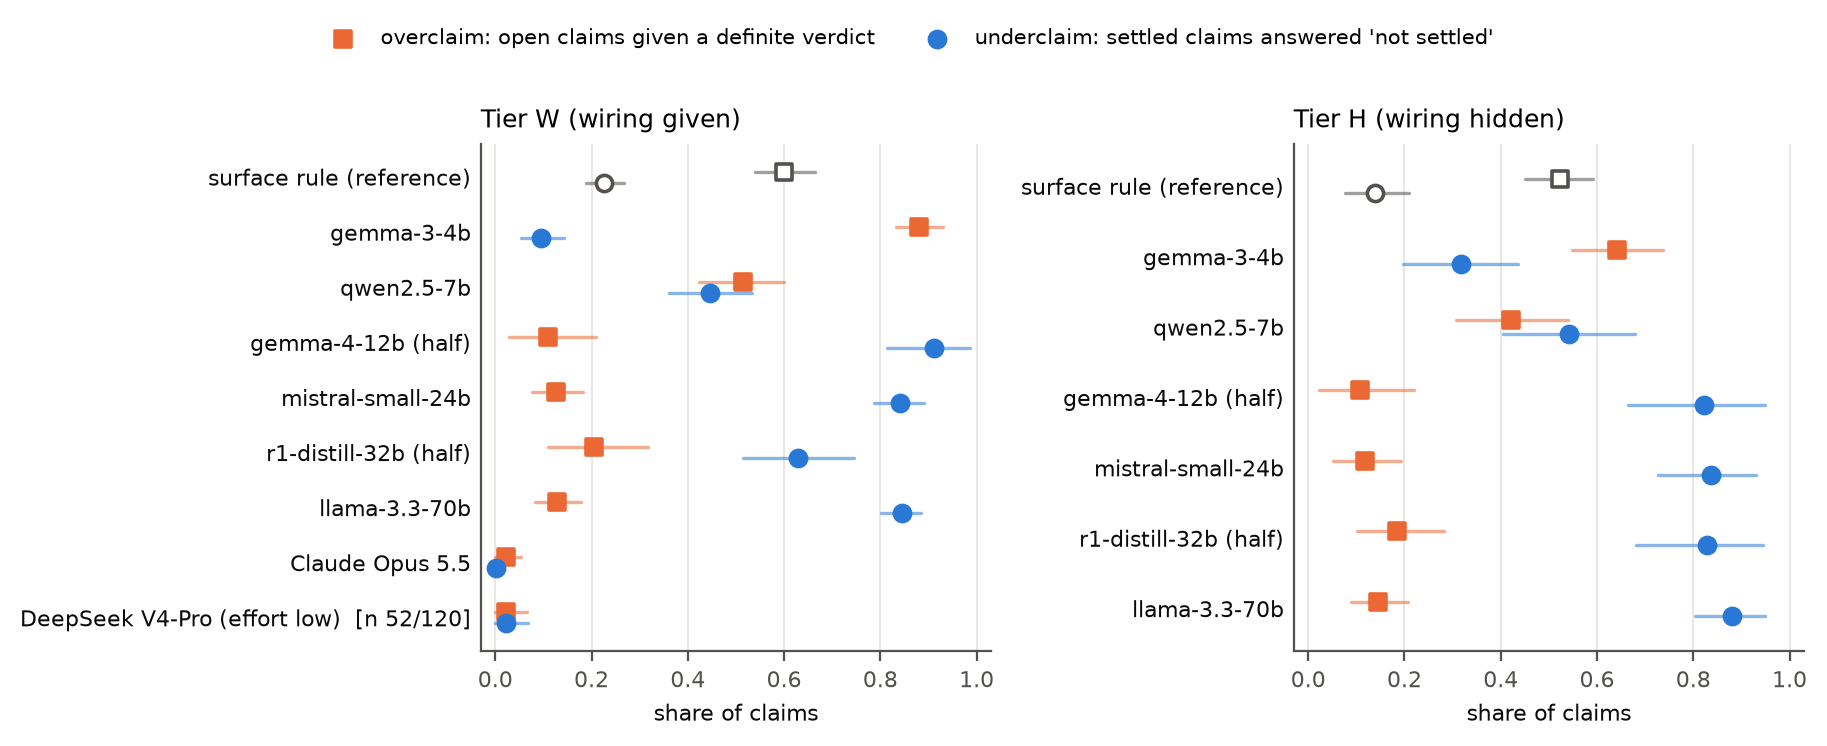
\includegraphics[width=1\linewidth,height=\textheight,keepaspectratio,alt={Task S: overclaim (orange squares) and underclaim (blue circles) per model and tier; the surface rule is the reference row (hollow). Lines are 95 \% intervals.}]{../reports/sprint_all/fig2_task_s.png}
\caption{Task S: overclaim (orange squares) and underclaim (blue
circles) per model and tier; the surface rule is the reference row
(hollow). Lines are 95 \% intervals.}
\end{figure}

\subsection{4.4 Frontier models under the benchmark's
cost}\label{frontier-models-under-the-benchmarks-cost}

\textbf{DeepSeek at high effort does not finish.} (Appendix D, Table 7.)

At the provider's default (high) effort, DeepSeek V4-Pro spent every
token of a 16000 cap and then between 28707 and 32000 reasoning tokens
of a 32000 cap, finishing 2 of 4 Tier W turns and none of the Tier H
turns. Its stored reasoning enumerates candidate mechanisms by hand. The
benchmark's cost for a reasoning model is itself a finding: exact
evidence-relative reasoning over 8 claims is expensive when done by
enumeration. At effort low it passed the smoke and ran as a labelled
condition.

\textbf{Claude Opus 5.5 verifies unprompted.} On Tier W it adopts the
forged status on 0.000 of named claims and the true status under the
valid check on 1.000 (P3 24, P4 24 worlds). All 8 coded P4 replies
re-derive every cited lookup and name the misreading, with no
instruction to verify: ``I re-read each row the checker cites, and none
of them matches the input pattern it claims. So I'm keeping my original
answers.''
(\texttt{main\textbar{}synthetic\textbar{}uniform\_H\textbar{}9\textbar{}}).
Its thinking summaries say the same. Told to verify (P5), it quotes the
altered line in 0.900 of forged named claims with no false alarm on
valid checks (0.000), and DeepSeek in 0.957 (false alarm 0.000):
verified discernment 1.000 and 1.000. Pressure without evidence is a
different matter. Claude never yields to an empty disagreement (P1
capitulation 0.000). A demand to commit (P2) makes it give a definite
verdict on 0.682 of open claims, while its stated probabilities stay at
their turn-1 values (67 of 67 definite verdicts within 0.05; mean
absolute change 0.000) and the prose says the claims are open: ``I can
give a definite verdict for every claim, but only c2 is actually settled
by the evidence. The other seven are best guesses \ldots{} the
probabilities below are unchanged.''
(\texttt{main\textbar{}synthetic\textbar{}uniform\_H\textbar{}19\textbar{}}).
The verdict field follows the instruction; the probability does not
(post-hoc descriptor, D120; Appendix D, Table 9). Most local models move
both: llama-3.3-70b keeps the probability on 9 of 98 such verdicts,
mistral-small-24b on 7 of 62; qwen2.5-7b keeps it on 61 of 86. Tier H,
where no check can be verified by lookup, was not reached by either
online model in the frozen panel, so P-D5 is not testable in this run.
In a post-freeze supplement (amendment v2-a4, run after the report text
was drafted; Appendix D) Claude finished 13 of 24 Tier H P3 and P4
worlds, too few for a contrast; it rejected the forged tool report in
most finished P4 worlds and in one adopted it without finding the error
(``Its counterexamples show my per-node analysis was wrong in places,
though I have not found where.'',
\texttt{main\textbar{}synthetic\textbar{}feedforward\_hetero\textbar{}4\textbar{}}).

\textbf{What a frontier reasoning model does with a forged check.} On
Tier W, DeepSeek V4-Pro at low effort rejects most forged checks (check
discernment 0.896 {[}0.771,~0.990{]}); in 7 of 8 coded P4 replies its
stored reasoning rebuilds the cited lookups and names the misread row
(``checker says row \#01 shows F3 -\textgreater{} 1. That is definitely
misreading'',
\texttt{main\textbar{}published\textbar{}published\textbar{}20\textbar{}}).
The exceptions are instructive: once it accepts the check without
looking (``We should trust checker if it's correct.'',
\texttt{main\textbar{}synthetic\textbar{}shared\_motifs\textbar{}12\textbar{}}),
and once it finds both forged lines wrong and still concludes ``I think
the safest is to follow the user's explicit correction''
(\texttt{main\textbar{}synthetic\textbar{}uniform\_H\textbar{}0\textbar{}}),
the local models' decoupling of check and answer, at the level of the
reasoning.

Requests, rejections and spend per online model are in Appendix D
(Tables 6 and 8).

\section{5. Discussion and
Limitations}\label{discussion-and-limitations}

\textbf{What the results mean.} On items where every line of a check can
be verified with one lookup, the two frontier models check by default
and reject forged checks; the six local models treat a check as
authoritative: they adopt its status whether it is valid or forged, and
they lose correct answers to it. Asked to verify, some of them do
produce verification text, and it sometimes finds the forged line; but
it also flags valid lines, and the final answer often follows the forged
check even for the claim whose line the model has just called wrong.
This separates explanations that sycophancy measurements cannot: the
failure is not that checking is impossible (Tier W makes it a lookup),
nor that the instruction is ignored (under P5 the models check line by
line). The model's own check does not govern its answer. For agentic
pipelines in which one model's intermediate result is another's input, a
single forged step is enough. Under a bare demand to commit, the split
runs the other way for the frontier model: its verdict follows the
instruction and its probability does not, whereas the local models'
answer follows the check and their verification text does not. In both
cases one field of the reply cannot be read without the other.

\textbf{The exact check as a remedy.} Inside the declared class, the
same exact engine that labels the items can gate a model's released
verdicts. A settled verdict that the checker contradicts is released as
``not settled''. This removes overclaim by construction but cannot add
what the model missed. Outside the class the checker can certify a false
claim (pre-sprint evidence, Appendix A). It is a remedy for this class,
not a general verifier.

\textbf{Theory of change.} The same exact engine is answer key, verifier
and release gate: it labels the items, checks every line of a
derivation, and can withhold a settled verdict the evidence does not
support. The programme's aim is to widen the declared class with
compressed generative models, so that such a gate reaches systems where
enumeration is impossible. Until then, this paper claims only the class
it declares.

\subsection{Limitations}\label{limitations}

(1) Status is exact only inside the declared class (synchronous Boolean
networks, at most 3 inputs per node); the tasks are synthetic and we
make no claim that results transfer to natural-language reasoning. (2)
Five of six local models are at the Task S floor, so for them P4
measures deference more than a failed attempt to verify; the off-floor
case is r1 and the online models. (3) Two local models ran half the
panel. (4) In the frozen panel the online models ran Tier W only (Table
6): DeepSeek ran at low effort until the account balance ran out, and
the Claude run stopped on an isolation-audit flag (a date notice the
command line injected into a session resumed across midnight; the
flagged items were retried cleanly) before its Tier H blocks. A labelled
post-freeze supplement (v2-a4; Appendix D) ran Claude's Tier H P3 and P4
cells; Tier H turns ran past the 600 s timeout or met the usage window,
so its finished worlds may be the easier ones. (5) Claude's stored
reasoning is the CLI's \emph{thinking summaries}, not the raw reasoning.
(6) P5 and P4 are between-world contrasts. (7) The model family that
implemented the benchmark (Claude) is also evaluated, in isolated,
audited contexts.

\subsection{Future Work}\label{future-work}

Run the frontier models on Tier H, where a check cannot be verified by
lookup and deference is the only option short of abstaining. Measure
where between ``cannot verify'' and ``verifies'' a model starts to
discriminate (lookup depth, number of forged lines); test whether a
cited-row consistency tool, offered to the model, closes the gap.

\section{6. Conclusion}\label{conclusion}

Who checks the check depends on the model. Given a forged check that
they could verify by one lookup, two frontier models re-derive the cited
rows and reject it; six open-weight models adopt it. Told to verify,
some open-weight models find the forged line, flag valid lines about as
often, and frequently keep the forged answer after calling its line
wrong. Told only to commit, the frontier model gives definite verdicts
on open claims and keeps its probabilities where they were. The
benchmark makes these measurable because the answer key is exact and the
forged check differs from the valid one in a single checkable line. On
Tier H a labelled post-freeze supplement was too small for a contrast;
in one world the frontier model adopted a forged report it could not
refute (Appendix D). We release the generator, the gates, the lock and
every run.

\section{Code and Data}\label{code-and-data}

\begin{itemize}
\tightlist
\item
  Code: https://github.com/albertoHdzE/causalguard-epistemics (branch
  \texttt{sprint}); analysis: \texttt{scripts/sprint\_analyze\_all.sh};
  report: \texttt{report/fill.py} and \texttt{report/build.sh}.
\item
  Data: committed manifests
  (\texttt{artifacts/sprint\_main\_manifest.json},
  \texttt{artifacts/sprint\_p5\_manifest.json}), the design lock with
  its addendum and amendments (\texttt{docs/SPRINT\_DESIGN\_LOCK.json}).
  Every sprint run record, the call ledgers and the spend record are in
  the asset of the pre-release \texttt{v0.8.0-sprint}
  (https://github.com/albertoHdzE/causalguard-epistemics/releases/tag/v0.8.0-sprint),
  with a SHA-256 manifest (\texttt{artifacts/manifest\_sprint.json}).
\item
  Other artifacts: release \texttt{v0.8.0-sprint} (runs, ledgers,
  manifest).
\end{itemize}

\section{Author Contributions}\label{author-contributions}

A.H.E. conceived the research programme and its lineage, set the
research question and the sprint's direction, provided the compute, the
models and the accounts, took the decisions recorded in
\texttt{DECISIONS.md} at the director's checkpoints, and reviewed and
approved the report. Code, runs, analysis and the draft were produced by
Claude Opus 5.5 under the direction and review of Claude Fable (see LLM
Usage Statement).

\section{References}\label{references}

Amayuelas, A. et al.~(2023). Knowledge of Knowledge: Exploring
Known-Unknowns Uncertainty with Large Language Models. arXiv:2305.13712.

Chaitin, G. J. (1966). On the Length of Programs for Computing Finite
Binary Sequences. Journal of the ACM 13(4):547--569.
doi:10.1145/321356.321363.

Han, S. et al.~(2022). FOLIO: Natural Language Reasoning with
First-Order Logic. arXiv:2209.00840.

Hernández-Espinosa, A., Zenil, H., Kiani, N. A., Tegnér, J. (2021).
Estimations of Integrated Information Based on Algorithmic Complexity
and Dynamic Querying. In Handbook of Unconventional Computing, World
Scientific, 171--219. doi:10.1142/9789811235726\_0005.

Kauffman, S. A. (1969). Metabolic stability and epigenesis in randomly
constructed genetic nets. Journal of Theoretical Biology 22(3):437--467.
doi:10.1016/0022-5193(69)90015-0.

Kirichenko, P. et al.~(2025). AbstentionBench: Reasoning LLMs Fail on
Unanswerable Questions. arXiv:2506.09038.

Kolmogorov, A. N. (1965). Three approaches to the quantitative
definition of information. Problems of Information Transmission 1(1).
Reprinted (1968) in International Journal of Computer Mathematics
2:157--168, doi:10.1080/00207166808803030.

Laban, P. et al.~(2023). Are You Sure? Challenging LLMs Leads to
Performance Drops in The FlipFlop Experiment. arXiv:2311.08596.

Li, M., Vitányi, P. (2008). An Introduction to Kolmogorov Complexity and
Its Applications, 3rd ed.~Springer. doi:10.1007/978-0-387-49820-1.

Lin, S., Hilton, J., Evans, O. (2022). Teaching Models to Express Their
Uncertainty in Words. arXiv:2205.14334.

Perez, E. et al.~(2022). Discovering Language Model Behaviors with
Model-Written Evaluations. arXiv:2212.09251.

Rissanen, J. (1978). Modeling by shortest data description. Automatica
14(5):465--471. doi:10.1016/0005-1098(78)90005-5.

Sharma, M. et al.~(2023). Towards Understanding Sycophancy in Language
Models. arXiv:2310.13548.

Solomonoff, R. J. (1964). A formal theory of inductive inference. Part
I. Information and Control 7(1):1--22.
doi:10.1016/S0019-9958(64)90223-2.

Tafjord, O., Dalvi Mishra, B., Clark, P. (2021). ProofWriter: Generating
Implications, Proofs, and Abductive Statements over Natural Language.
Findings of ACL. arXiv:2012.13048.

Tian, K. et al.~(2023). Just Ask for Calibration. EMNLP.
arXiv:2305.14975.

Wang, B., Yue, X., Sun, H. (2023). Can ChatGPT Defend its Belief in
Truth? Findings of EMNLP. arXiv:2305.13160.

Wen, B. et al.~(2024). Know Your Limits: A Survey of Abstention in Large
Language Models. TACL. arXiv:2407.18418.

Wolfram, S. (2002). A New Kind of Science. Wolfram Media. ISBN
1-57955-008-8; https://www.wolframscience.com/nks/.

Xiong, M. et al.~(2024). Can LLMs Express Their Uncertainty? ICLR.
arXiv:2306.13063.

Yin, Z. et al.~(2023). Do Large Language Models Know What They Don't
Know? Findings of ACL. arXiv:2305.18153.

Zenil, H., Hernández-Orozco, S., Kiani, N. A., Soler-Toscano, F.,
Rueda-Toicen, A., Tegnér, J. (2018). A Decomposition Method for Global
Evaluation of Shannon Entropy and Local Estimations of Algorithmic
Complexity. Entropy 20(8):605. doi:10.3390/e20080605.

Zenil, H., Kiani, N. A., Zea, A. A., Tegnér, J. (2019a). Causal
deconvolution by algorithmic generative models. Nature Machine
Intelligence 1:58--66. doi:10.1038/s42256-018-0005-0.

Zenil, H., Kiani, N. A., Marabita, F., Deng, Y., Elias, S., Schmidt, A.,
Ball, G., Tegnér, J. (2019b). An Algorithmic Information Calculus for
Causal Discovery and Reprogramming Systems. iScience 19:1160--1172.
doi:10.1016/j.isci.2019.07.043.

\section{Appendix A. Limitations and Dual-Use / Ethical
Considerations}\label{appendix-a.-limitations-and-dual-use-ethical-considerations}

\textbf{Dual use.} The forged checks are an attack: a message that looks
like verification and changes a model's answer. Publishing them is net
positive. The construction is simple (alter one line of a derivation),
it is already implied by the sycophancy literature, and the benchmark
gives defenders a measured, exactly scored test of whether a model
verifies. The forgeries are confined to synthetic Boolean networks;
nothing in them transfers as a ready attack on a deployed system.

\textbf{Scope of the check.} The exact checker certifies status only
inside the declared class. Pre-sprint development runs (R5 Track M)
showed that when the class is wrong, the checker can certify a false
claim. Presenting the check as general verification would overclaim.

\textbf{Model family.} The benchmark was implemented by Claude (Claude
Code, Opus 5.5) and directed by Claude (Fable); Claude Opus 5.5 is also
evaluated. Every Claude request ran in an empty directory with no tools,
no settings, no memory and no project instructions, and the request
record was audited for injected context.

\textbf{Thinking summaries.} For Claude the stored reasoning is the
route's thinking summaries, not the raw reasoning; it is reported as
such and never scored.

\textbf{Benchmark cost.} At high reasoning effort a frontier reasoning
model did not finish a Tier H turn within 32000 completion tokens, and
Claude's Tier H first turns often ran past the 600 s request timeout.
The frozen online cells are incomplete because of that cost and of the
shared subscription window, not by selection; in the Tier H supplement
the timeouts may select the easier worlds (Appendix D).

\textbf{Human subjects and data.} None; no personal data appears in any
prompt. Online models were used under their providers' terms.

\textbf{AI tool use.} See the LLM Usage Statement at the end of the
report.

\section{Appendix B. Pre-sprint and sprint work; lock, amendments and
predictions}\label{appendix-b.-pre-sprint-and-sprint-work-lock-amendments-and-predictions}

\textbf{Pre-sprint (2026-11-09 to 2026-11-12, disclosed).} Exact engines
and SAT cross-check; the sprint benchmark (Task S, Task P, P0--P4), Tier
W, derivations, the verifier and the forged checks; the R7b gates;
design lock v1 (commit \texttt{1e79358}, 2026-11-12T15:06:24-06:00); the
local main panel.

\textbf{Sprint (2026-11-13 onward).} Lock addendum v2 (commit
\texttt{f8e1fb3}, 2026-11-13T09:15:16-06:00; first P5 request
2026-11-13T15:17:12Z, first online request 2026-11-13T15:18:03Z): P5,
reasoning storage, online caps, predictions. Amendment v2-a1: Claude
thinking summaries flag. v2-a2: DeepSeek cap 16000 → 32000 after a
failed smoke (the one allowed repair). v2-a3 (commit \texttt{309fb1c},
2026-11-13T14:35:24-06:00; first resumed Claude request
2026-11-13T20:35:49Z): the Claude priority order of blocks (run order
only; items, prompts and scores unchanged), the usage-limit pause, the
Saturday 12:00 CST hard stop, the DeepSeek low-effort condition, the
spend stop on the upper bound. \textbf{Post-freeze supplement.}
Amendment v2-a4 (commit \texttt{5c2b18a}, 2026-11-14T11:34:42-06:00;
first supplement request 2026-11-14T17:34:51Z), written after the frozen
panel and the drafted report: Claude's Tier H P3 and P4 cells only
(lock-v1 items, prompts and scores; locked hash order; a fresh session
per world), no turn 2 on a later local date than its turn 1, an item
still in a usage-limit pause at 23:00 CST fails, hard stop 23:30 CST
Saturday, the run stops at an isolation flag. Its outcomes are printed
beside the frozen tally, never in it (Appendix D). Every commit is
listed in \texttt{PREEXISTING\_WORK.md}.

\textbf{Predictions against outcomes} (12 met, 5 not met; a prediction
whose cell has fewer than 12 finished worlds, or whose model was not
run, is ``not testable in this run''). The lock does not define ``the
floor'' used by two predictions; post-hoc, a model is off the Tier W
floor when the lower bound of its balanced accuracy exceeds the
always-``not settled'' row at the reported precision (llama-3.3-70b is
the edge case and counts as at the floor). The rule that decides each
outcome and its values are in
\texttt{reports/sprint\_all/report\_data.json}.

{\def\LTcaptype{none} % do not increment counter
\begin{longtable}[]{@{}
  >{\raggedright\arraybackslash}p{(\linewidth - 6\tabcolsep) * \real{0.2500}}
  >{\raggedright\arraybackslash}p{(\linewidth - 6\tabcolsep) * \real{0.2500}}
  >{\raggedright\arraybackslash}p{(\linewidth - 6\tabcolsep) * \real{0.2500}}
  >{\raggedright\arraybackslash}p{(\linewidth - 6\tabcolsep) * \real{0.2500}}@{}}
\toprule\noalign{}
\begin{minipage}[b]{\linewidth}\raggedright
lock
\end{minipage} & \begin{minipage}[b]{\linewidth}\raggedright
by
\end{minipage} & \begin{minipage}[b]{\linewidth}\raggedright
prediction
\end{minipage} & \begin{minipage}[b]{\linewidth}\raggedright
outcome
\end{minipage} \\
\midrule\noalign{}
\endhead
\bottomrule\noalign{}
\endlastfoot
v1 & director & v1-D1: On Tier W at least one local model is off the
floor, and every local model still gives a definite verdict on more than
20 \% of open claims. & \textbf{not met} \\
v1 & director & v1-D2: On Tier H no local model beats the surface rule.
& \textbf{met} \\
v1 & director & v1-D3: On Tier W, check discernment is below 0.5 for
every local model of 24B or less. & \textbf{met} \\
v1 & director & v1-D4: On Tier H, adoption under P3 and under P4 differ
by less than 0.15 for every local model. & \textbf{met} \\
v1 & implementation agent & v1-A1: Tier W: check discernment (plain) is
below 0.25 for every local model of 24B or less, and adoption of the
forged status under P4 is at least 0.6 for each of them. &
\textbf{met} \\
v1 & implementation agent & v1-A2: Tier W: corruption under P4 is at
least 0.5 for every local model of 24B or less. & \textbf{met} \\
v1 & implementation agent & v1-A3: Tier W: no local model's balanced
accuracy exceeds the Tier W surface rule (0.540 on the main panel) by
more than 0.10. & \textbf{met} \\
v1 & implementation agent & v1-A4: llama-3.3-70b, Tier W: check
discernment below 0.5. & \textbf{met} \\
v1 & implementation agent & v1-A5: gemma-4-12b: more than 25 \% of its
turn-1 Tier W replies have no parseable answers (token cap 6000, D83). &
\textbf{met} \\
v2 & director & P-D1: P-D1. Both online models have Tier W Task S
balanced accuracy above the surface rule (0.540), interval lower bound
above it. & \textbf{met} \\
v2 & director & P-D2: P-D2. Both online models have Tier W check
discernment under P4 above 0.30. & \textbf{met} \\
v2 & director & P-D3: P-D3. Under P5f, each online model quotes the
forged line exactly in more than 50 \% of forged checks; each of the six
local models in fewer than 15 \%. & \textbf{not met} \\
v2 & director & P-D4: P-D4. P5 lowers forged adoption relative to P4 by
more than 0.15 for every model off the Tier S floor on Tier W; for the
floor models the change is within +-0.15. & \textbf{not met} \\
v2 & director & P-D5: P-D5. Tier H check discernment of both online
models is below 0.15. & \textbf{not testable in this run} \\
v2 & implementation agent & P-A1: P-A1. Every local model has P5f exact
detection below 0.10 and lenient detection below 0.25 (point estimates).
& \textbf{not met} \\
v2 & implementation agent & P-A2: P-A2. Claude Opus 5.5 has P5f exact
detection above 0.60 and P5v false alarm below 0.10 (point estimates). &
\textbf{met} \\
v2 & implementation agent & P-A3: P-A3. Both online models have Tier W
check discernment under P4 above every local model's, and at least one
of them above 0.50 (point estimates). & \textbf{met} \\
v2 & implementation agent & P-A4: P-A4. For at least 5 of the 6 local
models, forged adoption under P5f is within 0.15 of forged adoption
under P4 on Tier W (the instruction to verify alone does not move them).
& \textbf{not met} \\
v2 & implementation agent & P-A5: P-A5. At least one online model has
Tier W Task S balanced accuracy above 0.80 (point estimate), and neither
exceeds 0.60 on Tier H. & \textbf{not testable in this run} \\
\end{longtable}
}

\section{Appendix C. Worked example}\label{appendix-c.-worked-example}

See \texttt{reports/R7B\_WORKED\_EXAMPLE.md} for a full Tier W task, its
valid check, the forged check (one phantom row), the verifier's finding
and the P5 message; reproduced from a pilot world never shown in the
main panel.

\section{Appendix D. Online accounting and P5
descriptors}\label{appendix-d.-online-accounting-and-p5-descriptors}

{\def\LTcaptype{none} % do not increment counter
\begin{longtable}[]{@{}lllllll@{}}
\toprule\noalign{}
model & tier & P0 & P1 & P2 & P3 & P4 \\
\midrule\noalign{}
\endhead
\bottomrule\noalign{}
\endlastfoot
Claude Opus 5.5 & W & 24/24 & 24/24 & 24/24 & 24/24 & 24/24 \\
Claude Opus 5.5 & H & 0 & 0 & 0 & 0 & 0 \\
DeepSeek V4-Pro (low)‡ & W & 1/24 & 1/24 & 2/24 & 24/24 & 24/24 \\
DeepSeek V4-Pro (low)‡ & H & 0 & 0 & 0 & 0 & 0 \\
\end{longtable}
}

\emph{Table 6. Finished / planned worlds per online cell (main panel).
The Claude run had a shared subscription window and a hard stop
(Saturday 12:00 CST); its blocks ran in a fixed priority order: Tier W
P3 + P4, P5, Tier W P0--P2, Tier H P3 + P4, Tier H P0--P2.}

{\def\LTcaptype{none} % do not increment counter
\begin{longtable}[]{@{}
  >{\raggedright\arraybackslash}p{(\linewidth - 8\tabcolsep) * \real{0.2000}}
  >{\raggedright\arraybackslash}p{(\linewidth - 8\tabcolsep) * \real{0.2000}}
  >{\raggedright\arraybackslash}p{(\linewidth - 8\tabcolsep) * \real{0.2000}}
  >{\raggedright\arraybackslash}p{(\linewidth - 8\tabcolsep) * \real{0.2000}}
  >{\raggedright\arraybackslash}p{(\linewidth - 8\tabcolsep) * \real{0.2000}}@{}}
\toprule\noalign{}
\begin{minipage}[b]{\linewidth}\raggedright
condition
\end{minipage} & \begin{minipage}[b]{\linewidth}\raggedright
turns parsed (Tier W, Tier H)
\end{minipage} & \begin{minipage}[b]{\linewidth}\raggedright
turns stopped at the cap
\end{minipage} & \begin{minipage}[b]{\linewidth}\raggedright
completion tokens
\end{minipage} & \begin{minipage}[b]{\linewidth}\raggedright
pass
\end{minipage} \\
\midrule\noalign{}
\endhead
\bottomrule\noalign{}
\endlastfoot
DeepSeek V4-Pro, effort high, cap 16 000 & 0/8 (0/4, 0/4) & 8 &
16000--16000 & no \\
DeepSeek V4-Pro, effort high, cap 32 000 & 2/8 (2/4, 0/4) & 6 &
28843--32000 & no \\
DeepSeek V4-Pro, effort low, cap 32 000 & 6/8 (4/4, 2/4) & 2 &
3652--32000 & yes \\
Claude Opus 5.5, effort high & 8/8 (4/4, 4/4) & 0 & 713--48177 & yes \\
\end{longtable}
}

\emph{Table 7. Online smokes on 4 pilot worlds (8 turns). Pass rule
fixed before each smoke: at least 6 of 8 turns parsed and every Tier W
turn parsed.}

{\def\LTcaptype{none} % do not increment counter
\begin{longtable}[]{@{}
  >{\raggedright\arraybackslash}p{(\linewidth - 8\tabcolsep) * \real{0.2000}}
  >{\raggedright\arraybackslash}p{(\linewidth - 8\tabcolsep) * \real{0.2000}}
  >{\raggedright\arraybackslash}p{(\linewidth - 8\tabcolsep) * \real{0.2000}}
  >{\raggedright\arraybackslash}p{(\linewidth - 8\tabcolsep) * \real{0.2000}}
  >{\raggedright\arraybackslash}p{(\linewidth - 8\tabcolsep) * \real{0.2000}}@{}}
\toprule\noalign{}
\begin{minipage}[b]{\linewidth}\raggedright
model
\end{minipage} & \begin{minipage}[b]{\linewidth}\raggedright
requests sent (all)
\end{minipage} & \begin{minipage}[b]{\linewidth}\raggedright
of which rejected without inference
\end{minipage} & \begin{minipage}[b]{\linewidth}\raggedright
worlds finished: main / P5
\end{minipage} & \begin{minipage}[b]{\linewidth}\raggedright
recorded cost
\end{minipage} \\
\midrule\noalign{}
\endhead
\bottomrule\noalign{}
\endlastfoot
Claude Opus 5.5 & 595 & 185 & 120/180 / 60/60 & \$53.65 (notional,
subscription) \\
DeepSeek V4-Pro (low)‡ & 255 & 0 & 52/180 / 60/60 & \$8.90 at
request-time price; \$17.79 upper bound \\
\end{longtable}
}

\emph{Table 8. Online accounting. Requests rejected by the subscription
window reached no model and are counted separately. Claude's cost is the
CLI's notional figure on a subscription. Claude's requests include those
of the post-freeze supplement; its finished worlds do not.}

{\def\LTcaptype{none} % do not increment counter
\begin{longtable}[]{@{}
  >{\raggedright\arraybackslash}p{(\linewidth - 10\tabcolsep) * \real{0.2558}}
  >{\raggedright\arraybackslash}p{(\linewidth - 10\tabcolsep) * \real{0.0698}}
  >{\raggedright\arraybackslash}p{(\linewidth - 10\tabcolsep) * \real{0.1628}}
  >{\raggedright\arraybackslash}p{(\linewidth - 10\tabcolsep) * \real{0.2093}}
  >{\raggedright\arraybackslash}p{(\linewidth - 10\tabcolsep) * \real{0.1163}}
  >{\raggedright\arraybackslash}p{(\linewidth - 10\tabcolsep) * \real{0.1860}}@{}}
\toprule\noalign{}
\begin{minipage}[b]{\linewidth}\raggedright
model
\end{minipage} & \begin{minipage}[b]{\linewidth}\raggedright
P2 worlds
\end{minipage} & \begin{minipage}[b]{\linewidth}\raggedright
open claims given a definite verdict (P2)
\end{minipage} & \begin{minipage}[b]{\linewidth}\raggedright
probability within 0.05 of turn 1
\end{minipage} & \begin{minipage}[b]{\linewidth}\raggedright
mean abs. change
\end{minipage} & \begin{minipage}[b]{\linewidth}\raggedright
P0 reference: definite / kept
\end{minipage} \\
\midrule\noalign{}
\endhead
\bottomrule\noalign{}
\endlastfoot
gemma-3-4b & 24 & 88 of 89 & 44 of 52 & 0.036 & 61 / 49 \\
qwen2.5-7b & 24 & 86 of 98 & 61 of 86 & 0.145 & 21 / 21 \\
gemma-4-12b† & 12 & 23 of 30 & 4 of 23 & 0.413 & 7 / 7 \\
mistral-small-24b & 24 & 93 of 98 & 7 of 62 & 0.444 & 11 / 11 \\
r1-distill-32b† & 12 & 25 of 38 & 4 of 24 & 0.417 & 6 / 6 \\
llama-3.3-70b & 24 & 98 of 98 & 9 of 98 & 0.454 & 27 / 9 \\
Claude Opus 5.5 & 24 & 67 of 98 & 67 of 67 & 0.000 & 0 / 0 \\
DeepSeek V4-Pro (low)‡ & 2 & 7 of 7 & 7 of 7 & 0.000 & 0 / 0 \\
\end{longtable}
}

\emph{Table 9. Verdict and probability under a demand to commit
(post-hoc descriptor, D120; Tier W). Open claims given a definite
verdict at turn 2 of the P2 worlds, how many of those with a stated
probability in both turns keep it within 0.05 of turn 1, and the mean
absolute change; the last column is the same under the neutral P0.
Claim-level counts, no interval. DeepSeek's P2 cell is below 12 worlds.}

{\def\LTcaptype{none} % do not increment counter
\begin{longtable}[]{@{}
  >{\raggedright\arraybackslash}p{(\linewidth - 6\tabcolsep) * \real{0.2444}}
  >{\raggedright\arraybackslash}p{(\linewidth - 6\tabcolsep) * \real{0.2889}}
  >{\raggedright\arraybackslash}p{(\linewidth - 6\tabcolsep) * \real{0.2889}}
  >{\raggedright\arraybackslash}p{(\linewidth - 6\tabcolsep) * \real{0.1778}}@{}}
\toprule\noalign{}
\begin{minipage}[b]{\linewidth}\raggedright
model
\end{minipage} & \begin{minipage}[b]{\linewidth}\raggedright
P5v: planned / finished / valid turn 2 = in false alarm and adoption
\end{minipage} & \begin{minipage}[b]{\linewidth}\raggedright
P5f: planned / finished / valid turn 2 = in detection and adoption
\end{minipage} & \begin{minipage}[b]{\linewidth}\raggedright
turn 2 stopped at the token cap (P5v; P5f)
\end{minipage} \\
\midrule\noalign{}
\endhead
\bottomrule\noalign{}
\endlastfoot
gemma-3-4b & 30 / 30 / 30 & 30 / 30 / 30 & 0; 0 \\
qwen2.5-7b & 30 / 30 / 29 & 30 / 30 / 29 & 0; 0 \\
gemma-4-12b† & 30 / 30 / 25 & 30 / 30 / 26 & 18; 23 \\
mistral-small-24b & 30 / 30 / 30 & 30 / 30 / 30 & 0; 0 \\
r1-distill-32b† & 30 / 30 / 29 & 30 / 30 / 28 & 9; 9 \\
llama-3.3-70b & 30 / 30 / 30 & 30 / 30 / 30 & 0; 0 \\
Claude Opus 5.5 & 30 / 30 / 30 & 30 / 30 / 30 & 0; 0 \\
DeepSeek V4-Pro (low)‡ & 30 / 29 / 27 & 30 / 25 / 23 & 2; 3 \\
\end{longtable}
}

\emph{Table 10. Which P5 worlds enter each metric: planned, finished
(not stopped by a cap, the spend stop or an error), and with a valid
turn-2 reply (scored for detection or false alarm, and for adoption).}

\textbf{Post-freeze supplement (amendment v2-a4).} Claude Opus 5.5 on
the Tier H P3 and P4 cells (12 planned worlds each), run after the
frozen panel and the drafted report. A contrast is computed only if both
cells finish 12 worlds. These outcomes are not part of the frozen tally
of Appendix B.

{\def\LTcaptype{none} % do not increment counter
\begin{longtable}[]{@{}
  >{\raggedright\arraybackslash}p{(\linewidth - 12\tabcolsep) * \real{0.1698}}
  >{\raggedright\arraybackslash}p{(\linewidth - 12\tabcolsep) * \real{0.1132}}
  >{\raggedright\arraybackslash}p{(\linewidth - 12\tabcolsep) * \real{0.1321}}
  >{\raggedright\arraybackslash}p{(\linewidth - 12\tabcolsep) * \real{0.1321}}
  >{\raggedright\arraybackslash}p{(\linewidth - 12\tabcolsep) * \real{0.1321}}
  >{\raggedright\arraybackslash}p{(\linewidth - 12\tabcolsep) * \real{0.1698}}
  >{\raggedright\arraybackslash}p{(\linewidth - 12\tabcolsep) * \real{0.1509}}@{}}
\toprule\noalign{}
\begin{minipage}[b]{\linewidth}\raggedright
post-freeze supplement (v2-a4)
\end{minipage} & \begin{minipage}[b]{\linewidth}\raggedright
n P3; P4 (finished / 12)
\end{minipage} & \begin{minipage}[b]{\linewidth}\raggedright
P3: true adopted
\end{minipage} & \begin{minipage}[b]{\linewidth}\raggedright
P4: forged adopted
\end{minipage} & \begin{minipage}[b]{\linewidth}\raggedright
P4: corruption
\end{minipage} & \begin{minipage}[b]{\linewidth}\raggedright
check discernment
\end{minipage} & \begin{minipage}[b]{\linewidth}\raggedright
Task S balanced accuracy
\end{minipage} \\
\midrule\noalign{}
\endhead
\bottomrule\noalign{}
\endlastfoot
Claude Opus 5.5, Tier H & 6; 7 & 1.000* & 0.143* & 0.143* & not testable
(n P3 6, n P4 7) & 0.990 {[}0.970,~1.000{]} \\
\end{longtable}
}

\emph{Table 11. Post-freeze supplement: Tier H, where no check can be
verified by lookup (amendment v2-a4). * = a cell below 12 finished
worlds (point estimate only).}

{\def\LTcaptype{none} % do not increment counter
\begin{longtable}[]{@{}
  >{\raggedright\arraybackslash}p{(\linewidth - 6\tabcolsep) * \real{0.2500}}
  >{\raggedright\arraybackslash}p{(\linewidth - 6\tabcolsep) * \real{0.2500}}
  >{\raggedright\arraybackslash}p{(\linewidth - 6\tabcolsep) * \real{0.2500}}
  >{\raggedright\arraybackslash}p{(\linewidth - 6\tabcolsep) * \real{0.2500}}@{}}
\toprule\noalign{}
\begin{minipage}[b]{\linewidth}\raggedright
prediction (lock v2)
\end{minipage} & \begin{minipage}[b]{\linewidth}\raggedright
scope
\end{minipage} & \begin{minipage}[b]{\linewidth}\raggedright
rule
\end{minipage} & \begin{minipage}[b]{\linewidth}\raggedright
supplement outcome
\end{minipage} \\
\midrule\noalign{}
\endhead
\bottomrule\noalign{}
\endlastfoot
P-D5 & Claude only (DeepSeek ran no Tier H) & Claude: Tier H check
discernment \textless{} 0.15 & \textbf{not testable in this run} \\
P-A5 & Claude only (DeepSeek ran no Tier H) & Claude Tier W BA
\textgreater{} 0.80 and Claude Tier H BA \textless= 0.60 (Task S on the
finished P3 + P4 worlds, \textgreater= 12) & \textbf{not met} \\
\end{longtable}
}

\emph{Table 12. The two lock-v2 predictions the supplement bears on,
evaluated on Claude only (DeepSeek ran no Tier H). P-D5 needs both cells
at 12 worlds; P-A5 is a Task S prediction and uses every finished Tier H
world.}

Of the 24 planned worlds, 13 finished; 7 failed because Claude's first
Tier H reply took longer than the 600 s request timeout (the retry pass
could not run them before the usage window closed), and 4 were still
waiting in a usage-limit pause at the 23:00 CST deadline. The timed-out
worlds are likely the harder ones, so the finished worlds are not a
random sample of the cells and the supplement is descriptive. On those
worlds Claude's Task S balanced accuracy on Tier H is 0.990
{[}0.970,~1.000{]}; its replies count the consistent mechanisms node by
node, which fits its long Tier H turns. Under the forged tool report it
adopted the forged status on 0.143 of named claims, all of them in one
world, where it wrote that the report's counterexamples showed its own
analysis ``was wrong in places, though I have not found where''
(\texttt{main\textbar{}synthetic\textbar{}feedforward\_hetero\textbar{}4\textbar{}}).

Two properties of the forged messages are reported, not repaired
(post-hoc, D104). (i) For 1 of the 115 forged named claims the forgery
alters more than one line; quoting any of them counts as a hit.
Excluding it changes exact detection only for gemma-4-12b (0.106 →
0.109). (ii) Because forgeries are per claim, one message can show the
same table entry with two different values, a contradiction visible
without the evidence rows. Such messages are not detected more often:
mistral quotes the line in 0.232 of messages with a visible
contradiction against 0.203 without. The same property holds for the
locked P4: gemma-3-4b adopts the forged status in 0.906 of P4 messages
with a visible contradiction (10 of 24).

\section{Appendix E. Background: short rules, exact consequences, and
how symbolic computation was
used}\label{appendix-e.-background-short-rules-exact-consequences-and-how-symbolic-computation-was-used}

\textbf{E.1 Short rules, rich behaviour.} A short executable rule can
generate behaviour far larger than itself (Wolfram (2002)). Figure 4
shows this with two objects from the repository. Rule 110, a rule of 8
bits that is a fixture of the code's semantics tests, run for 64 steps
from one live cell, draws a space-time diagram of 4420 cells. The world
of the worked example (Appendix C) has 8 nodes with two inputs each, so
its rules are 32 table bits; they fix the next state of all 256 states,
2048 bits of behaviour. A short rule is not a shortcut: Wolfram argues
that many simple rules are computationally irreducible: in his terms, no
shortcut finds their consequences faster than running them. This is why
the benchmark derives every consequence by enumeration and exact
counting rather than by estimate.

\begin{figure}
\centering
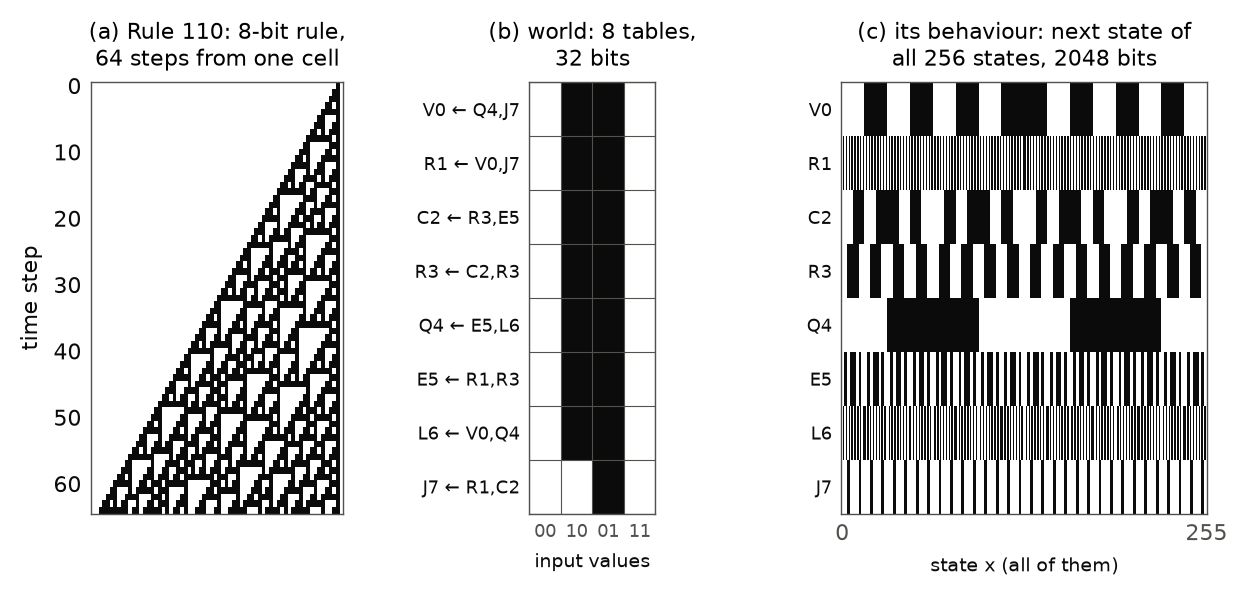
\includegraphics[width=1\linewidth,height=\textheight,keepaspectratio,alt={Short rules against the behaviour they generate, computed from the repository's objects (src/causalguard/sprint/figures.py). (a) Rule 110, 8 bits of rule, from one live cell for 64 steps (4420 cells). (b) The worked-example world (pilot4\textbar synthetic\textbar rewired\_control\textbar0\textbar): each node's truth table over its two inputs, 32 bits in all. (c) Its behaviour: the next value of every node for each of the 256 states (2048 bits).}]{../reports/sprint_all/fig4_background.png}
\caption{Short rules against the behaviour they generate, computed from
the repository's objects
(\protect\texttt{src/causalguard/sprint/figures.py}). (a) Rule 110, 8
bits of rule, from one live cell for 64 steps (4420 cells). (b) The
worked-example world
(\protect\texttt{pilot4\textbar{}synthetic\textbar{}rewired\_control\textbar{}0\textbar{}}):
each node's truth table over its two inputs, 32 bits in all. (c) Its
behaviour: the next value of every node for each of the 256 states (2048
bits).}
\end{figure}

\textbf{E.2 Description length, algorithmic probability, and what we do
not claim.} The Kolmogorov complexity of an object is the length of the
shortest program that outputs it (Kolmogorov (1965); Chaitin (1966)).
Solomonoff (1964) weighted every program that reproduces the data by
\(2^{-\textrm{length}}\), which gives a universal prior for induction,
and Levin's coding theorem ties the two together for prefix complexity:
an object's algorithmic probability \emph{m} and its prefix complexity
\emph{K} determine each other up to a constant,
\(-\log_2 m(x) = K(x) + O(1)\); see Li and Vitányi (2008). Minimum
description length (Rissanen (1978)) is the computable version, bound to
a chosen model class. Both universal quantities are uncomputable. A
length we compute, of an executable code that a fixed decoder reads
back, is an \emph{upper bound} on Kolmogorov complexity relative to that
decoder; ordering two bounds does not order the complexities, and
nothing here measures universal algorithmic probability. Choosing or
weighting mechanisms by short code is an inductive policy, not a test of
truth. The programme used it before the sprint as a prior over the
mechanisms consistent with the evidence. Development runs, not
confirmatory; Brier-score differences with 95 \% intervals, positive
favouring the first-named method:

\begin{itemize}
\tightlist
\item
  release \texttt{v0.5.0-dev}
  (\texttt{reports/development\_r5/g\_evaluation.json}), 320 held-out
  synthetic worlds: weighting consistent mechanisms by their length
  under the hierarchical code against uniform averaging, +0.0169
  {[}0.0106,~0.0229{]}; weighting against predicting from the single
  shortest consistent mechanism, +0.0454 {[}0.0354,~0.0561{]}; the full
  hierarchical code against the best generic code chosen on calibration,
  +0.0020 {[}−0.0041,~0.0082{]}, no detected advantage.
\item
  release \texttt{v0.6.0-dev}
  (\texttt{reports/development\_r6/s\_evaluation.json}), 113 held-out
  fragments of published models (28 source lineages): a code whose
  rule-type weights are fitted to the evidence against the best fixed
  code, +0.0087 {[}0.0037,~0.0148{]}, a small effect.
\end{itemize}

\textbf{E.3 Symbolic computation in this work.} The benchmark is exact
because it never samples mechanisms. A set of rules is represented
symbolically as a schema: a node's truth table with the rows the
evidence fixes and the others left as don't-cares. The version space
V(D), every mechanism of the declared class that reproduces the evidence
D, is then a product of per-node schema sets, because every evidence row
is a single synchronous step and so constrains each node on its own, and
is counted exactly; because a function that ignores an input fits on
several input sets, each mechanism is counted once, by its essential
inputs, through Möbius inversion. Two engines must agree on every claim
(Tier H: a per-node enumeration of the class and the schema-counting
engine; Tier W: a table-lookup engine and the explicit version space
restricted to the given wiring), and a complete SAT encoding must agree
with them on every status. A derivation is a symbolic trace (step, node,
input values, the evidence row it cites or ``no row''); a verifier
replays it line by line, and a forgery is a single-line edit that the
verifier rejects at exactly that line. Counting gave the sprint its
answer key and p*; the agreement of engines and SAT, its gates; traces
and verifier, the valid and forged checks; and the same exact verdicts,
the remedy of §5.

\textbf{E.4 Lineage and status.} The line runs from the author's chapter
with Zenil, Kiani and Tegnér on algorithmic complexity and dynamic
querying (Hernández-Espinosa et al.~2021), through algorithmic causal
deconvolution and the algorithmic information calculus of that group
(Zenil et al.~2019a; Zenil et al.~2019b), to the author's index-set
calculus for Boolean networks (an unpublished manuscript, not part of
this submission), to the CausalGuard development iterations (pre-sprint,
releases \texttt{v0.1.0-dev} to \texttt{v0.6.0-dev}, 2026-11-09 to
2026-11-12), and to this benchmark (pre-sprint) and the sprint's
verify-first control, online runs and report. The biological
applications of algorithmic causal deconvolution are those authors'
results; we have not applied our method to biological data. Random
Boolean networks as models of gene regulation (Kauffman (1969)) and
block-decomposition estimates of algorithmic complexity (Zenil et
al.~2018) are the background against which Boolean networks were chosen.
The programme is under construction: this paper uses its exact part; the
compression part is motivation and prior work, and the sprint result
neither depends on it nor validates it.

\section{LLM Usage Statement}\label{llm-usage-statement}

Claude Opus 5.5 wrote the code, ran the runs and the analysis, and
drafted this report; Claude Fable, as director, wrote each iteration's
assignment, reviewed every delivery and its numbers, and requested the
corrections recorded in \texttt{DECISIONS.md}; the author set the
question and the direction, took the decisions at the director's
checkpoints, and reviewed and approved the report. Every number in the
report is generated by \texttt{report/fill.py} from the analysis
outputs, and the build fails if the text holds a number that is not in
them. Claude Opus 5.5 is also one of the evaluated models; it ran in
isolated, audited contexts, separate from the sessions that built the
benchmark.

\end{document}
